\chapter{Experiments and results}
\label{ch:experiments_and_results}

\begin{flushright}
\rightskip=.8cm\textit{``To apply oneself to great inventions, starting from the smallest beginnings, is no task for ordinary minds; to divine that wonderful arts lie hid behind trivial and childish things is a conception for superhuman talents.''} \\
\vspace{.2em}
\rightskip=.8cm Galileo Galilei
\end{flushright}
\vspace{1em}


There exists many works in literature regarding controllable content generation, although most of them involve procedural generation with models different from ANNs, such as multi-dimensional Markov chains \cite{markov}. Unfortunately, large constrained objects data sets to be used as a common benchmark for this task are still missing since many authors have not shared their data. For this reasons, all the experiments have been performed on synthetic data sets. For sure these results are not sufficient alone to prove the effectiveness of the proposed model on a wide range of applications, nevertheless programmatically generated data are useful to easily test specific design choices, especially in an early research stage.


\section{Data sets}

All the experiments have been performed on two similar data sets. To each of them is assigned a label by which they can be easily later referred to.

The first data set is composed of $23,040$ black-and-white square images of $20$x$20$ pixel. The training set is made up of $18,944$ items, while the test set of the remaining $4,096$ items. Each image contains exactly two different white regular polygons randomly chosen among triangles $(30\%)$, squares $(30\%)$ and rhombi $(40\%)$. Each polygon has an area of exactly 25 pixels. Polygons are randomly placed on a black background without overlapping and avoiding the outer border. This data set is labelled as \textit{poly20}.

\begin{figure}
    \centering
    \begin{minipage}{0.45\textwidth}
        \centering
        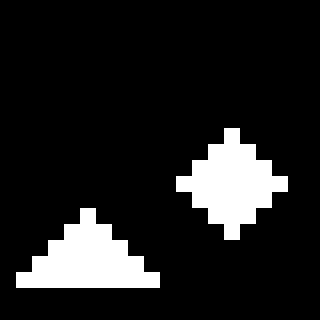
\includegraphics[width=0.6\textwidth]{poly20_zoom}
        \caption{Sample from \textit{poly\_20} (zoom).}
    \end{minipage}
    \hfil
    \begin{minipage}{0.45\textwidth}
        \centering
        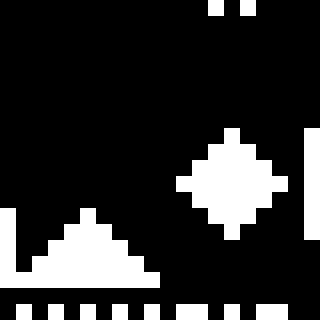
\includegraphics[width=0.6\textwidth]{poly20_pc_zoom}
        \caption{Sample from \textit{poly\_20\_pc} (zoom).}
    \end{minipage}
\end{figure}

The second data set is identical to the first but for the usage of the pixels on the outer border. Each of them now represents a \textit{parity check} of other close inner pixels. In particular, a pixel lying on a vertical border (left or right) will be the parity check of the $9$ inner nearest pixels lying on the same row (left-half or right-half). Similarly, a pixel lying on a horizontal border (top or down) will be the parity check of the $9$ inner nearest pixels lying on the same column (top-half or bottom-half). By assigning the values of $0$ and $1$ to, respectively, black and white pixels, we can formally describe the borders of a matrix-like image $I$:

\begin{equation}
\label{eq:parity_check}
\forall i = 1, ..., 20: 
\begin{cases}
     I[i][0] = \sum\limits_{k=2}^{10} I[i][k] \mod 2 & \text{(bottom-half columns)} \\
     I[i][20] = \sum\limits_{k=11}^{19} I[i][k] \mod 2 & \text{(top-half columns)} \\
     I[0][i] = \sum\limits_{k=2}^{10} I[k][i] \mod 2 & \text{(left-half rows)} \\
     I[20][i] = \sum\limits_{k=11}^{19} I[k][i] \mod 2 & \text{(right-half rows)} \\
\end{cases}.
\end{equation}

The second data set is labelled as \textit{poly20\_pc}.

\begin{figure}[ht]
    \centering
    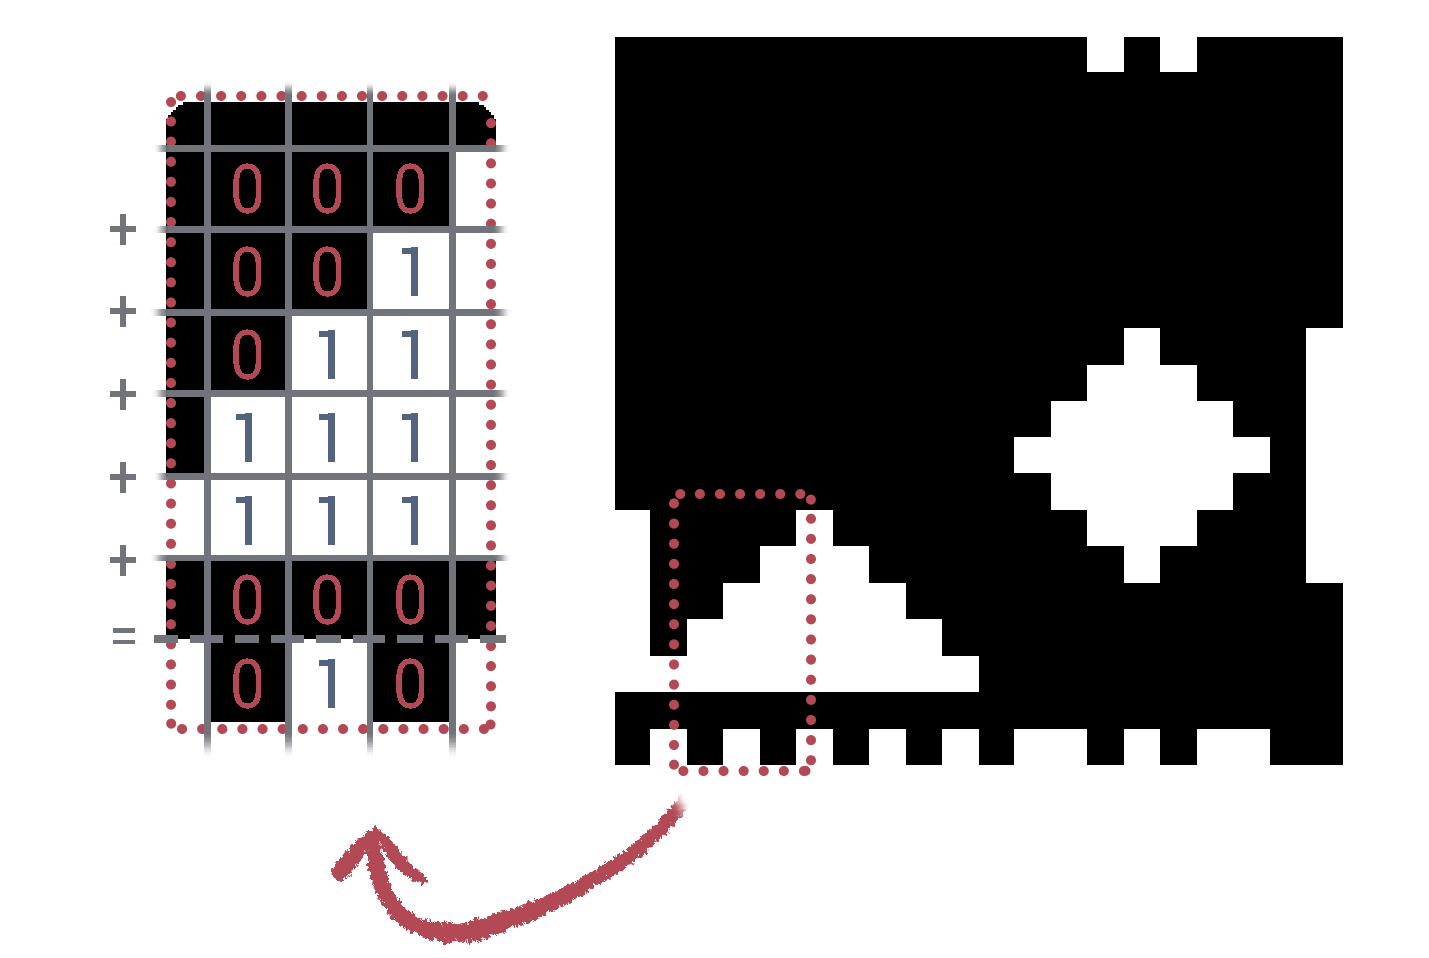
\includegraphics[width=0.7\textwidth]{pc_zoom}
    \caption{Schematic representation of how parity checks are computed.}
\end{figure}

The two data sets have been generated according to the following criteria:

\begin{itemize}
    \item the number of items in the data sets is as large as possible, yet bounded by the constraints on the polygons area and their non-overlapping placement;
    \item small $20$x$20$ pixel images allow a faster training with modest-size ANNs architectures that comes handy in an exploratory research scenario;
    \item placing two polygons on each image, instead of a single one, avoids the \textit{mode collapsing problem} of GANs. In fact, by doing so, the generator can not try to learn only the easiest shape, that is the one more frequently classified as a training datum by the discriminator. Instead, it is continually forced to learn combinations of them and, consequently, each of them. This evidence is the result of some preliminary experiments on GANs;
    \item rhombi are supposed to be the most difficult polygons to learn among the three available, so they are slightly more present in the data sets;
    \item the constant value of $25$ for the polygons area maximises the number of convex regular polygons that can be discretely represented;
    \item each parity check is computed only on one half of the image to model a function of modest complexity. If desired, these constraints can become harder by extending them on entire rows/columns.
\end{itemize}


A final note regards the choice of parity check pixels in \textit{poly20\_pc}. Their goal is to dramatically reduce the probability for the generator to output a perfect object without having first learnt the rules that define the border of the images. Each parity check, in fact, halves the probability to generate by chance a perfect object. In this way, the generator is forced to learn the relations expressed in \eqref{eq:parity_check}. Furthermore, from a computational point of view, checking if a pixel is correct is very fast. Hence, parity checks seem a suitable family of functions to test the proposed deep generative model: functions that are hard to learn and easy to verify.


\section{Model implementation}

The deep generative framework is implemented in Python and will be open-sourced. The input of the software is a JSON file describing the experiment to be run. It contains information about the data set to be generated or reused, the ANNs architectures and some training parameters and hyperparameters. Every descriptor is thus sufficient to train and evaluate the entire model. Experiments are deterministic and reproducible since JSON files also contain the seeds for the random distributions.

ANNs are trained using TensorFlow \cite{tensorflow}, the open-source ML framework developed by Google. The experiment descriptor includes function names to be used to build the model, together with references to the loss function and the optimization algorithm.

The JSON file can optionally contain a list of constraints. If provided, the resulting generative model will be that of CANs, otherwise simple BGANs. In the first case, constraints will be used during training according to the ANN model specified.

To reduce execution times, penalty functions are dynamically compiled to native machine instructions with Numba \cite{numba}   and they are evaluated in parallel on sampled data by all available CPU cores, avoiding Python's Global Interpreter Lock. In addition, generated samples are also independent of each other, so they can be further processed in parallel in a thread-safe way. On the contrary, data sets penalty vectors are computed once, at the beginning of the training algorithm, and cached, since their values never change. As a result, this single-GPU/multi-core implementation provides similar running times for BGANs and CANs.

Statistics are collected during the training mainly via TensorBoard, the native visualization tool tightly integrated with TensorFlow. This is the best solution to get insights on the training process since some parts of the computation are compiled for the GPU and not exposed via any API. Statistics can be collected with a customized frequency both on the validation set and on the test set.


\section{Experimental protocol}


Probabilistic generative models can be used for many different tasks, such as compression, denoising, semi-supervised learning or unsupervised feature learning. Given this wide range of applications, a lot of heterogeneity exists in the way these models are trained and evaluated. Some works have proved that good performance with respect to one criterion do not imply good performance with respect to other criteria \cite{evaluation}. Since being able to generate realistic samples from the data distribution
is one of the goals of a generative model, sometimes they are simply evaluated by visually inspecting the samples. Typically, the evaluation is carried out by experimental subjects who do not know the source of the samples \cite{human_evaluators}. Unfortunately, it is possible for a very poor probabilistic model to produce very good samples. However, the framework of this work enables an objective evaluation via penalty functions and no subjective assessment is necessary.

ANNs generally require a significative amount of random numbers to be trained. They are used, for instance, to initialize the weights of the network or to randomly shuffle mini-batches before every new training epoch. GANs-based models, in particular, involve a far greater amount of noise, since new vectors are required to sample data from $p_g$ and this operation is usually performed a million times. However, due to computational implications, extensively testing ANNs can be really time-consuming and it can be hard to get results with a high significance level.

Experiments have been repeated multiple times with different random seeds. Each plot shows the number of repetitions and highlights the first, second and third quartiles of the aggregated results regarding the performance measure of interest.

Networks have been evaluated for their capability to satisfy constraints individually and simultaneously. In the first case, plots show the average over all constraints of the percentages of objects satisfying each of them. In the latter, they show the percentage of perfect objects produced. In both cases, the images involved in the measurement are those generated during a training epoch on the test set after which no optimization is performed.

The tested BGANs and CANs architectures are equivalent, with the obvious exception of the hidden units reserved for the constraints, that are CANs-specific. Networks are also initialized in the same way and visually evaluated on the same input noise. To measure their capability of generating objects satisfying constraints, a number of statistics are periodically collected during training, such as the percentage of perfect objects being generated or the mean error on each penalty function.

Stochastic optimization is performed via Adam \cite{adam} and batch normalization \cite{batch_norm} is used on some layers to accelerate training.

The reported execution times refer to the experiments performed on \textit{Maximillian Pegasus}\footnote{Lorenzo, thanks from the bottom of my heart.}: CPU Intel Core i$7$-$5930$K $3.5$GHz, $6$ cores; $3$x GPU MSI GeForce GTX $980$, $4$GB; RAM $16$GB; OS Windows $10$; Python version $3.5.2$; TensorFlow-GPU version $1.6.0$; Nvidia driver $391.01$; CUDA version $9.0$; cuDNN version $7.0.5$.


\section{Model architectures}

Not being interested in finding the best architecture for the task, but only in comparing BGANs and CANs with the same architecture, the experimentation does not involve model selection. On the contrary, the architecture initially adopted, together with all its hyperparameters, is the one described in the original work on BGANs. Preliminary works on BGANs have proved this architecture to have enough capacity to learn in a reasonable amount of time how to generate images of different kinds. Similarly to data sets, also architectures are labelled for convenience.

Generators and discriminators tend to have symmetric configurations. This choice makes the adversarial training procedure quite stable over the epochs and overall effective. Discriminator architectures usually involve convolutional layers to learn spatially local patterns of input polygons. Vice versa, generator architectures use the opposite operation, the transposed convolution layer, often simply called deconvolution, to expand input noise into meaningful shapes.

The following is a schematic description of the architectures. For each of them is provided the complete list of composing layers, along with their parameters and input/output dimensions. The symbol $\stackrel{r}{\to}$ is used to indicate reshaping operations. The symbol $\stackrel{t}{\to}$ represents a transpose operation. The symbol $\stackrel{c}{\to}$ denotes that the layer has been expanded to introduce hidden units to be fed with values computed by penalty functions.

The placeholder $?$ is used for input values. For generator architectures usually it is $|\bm{z}| \times |mini\text{-}batch|$, while for discriminator architectures it is $|samples| \times |mini\text{-}batch|$, where $|samples|$ represents the number of samples drawn for each generator output, as specified by BGANs. Default values are $|\bm{z}| = 64$, $|samples| = 20$, $|mini\text{-}batch| = 64$.


\begin{description}
\item \textit{bgan20\_gen}: generator network originally used for BGANs, adapted for 20x20 pixel data sets.
\begin{enumerate}
    \item $(?, 64) \to (?, 1024)$. Type: dense ($1024$ output units); activation: ReLU; batch normalization. 
    \item $(?, 1024) \to (?, 3200)$. Type: dense ($3200$ output units); activation: ReLU; batch normalization.
    \item $(?, 3200) \stackrel{r}{\to} (?, 5, 5, 128) \to (?, 10, 10, 64)$. Type: deconvolution; filters: 64; kernel size: 5; strides: 2; kernel initializer: orthogonal; bias initializer: zeros; activation: ReLU; batch normalization.
    \item $(?, 10, 10, 64) \to (?, 20, 20, 1)$. Type: deconvolution; filters: 1; kernel size: 5; strides: 2; kernel initializer: orthogonal; bias initializer: zeros; activation: linear.
   \end{enumerate}
\item \textit{bgan20\_discr\_h32l}: discriminator network similar to the one originally used for BGANs, adapted for 20x20 pixel data sets. Layer \ref{additional_layer} is added for consistency with the corresponding constrained discriminator layer reserved for penalty function values (\textit{can20\_discr\_h32l}, layer \ref{constrained_layer}).
\begin{enumerate}
    \item $(?, 20, 20, 1) \to (?, 10, 10, 64)$. Type: convolution; filters: 64; kernel size: 5; strides: 2; kernel initializer: Xavier; activation: leaky ReLU ($a = 0.2$).
    \item $(?, 10, 10, 64) \to (?, 5, 5, 128)$. Type: convolution; filters: 128; kernel size: 5; strides: 2; kernel initializer: Xavier; activation: leaky ReLU ($a = 0.2$).
    \item $(?, 5, 5, 128) \stackrel{r}{\to} (?, 3200) \to (?, 1024)$. Type: dense ($1024$ output units); kernel initializer: Xavier; activation: leaky ReLU ($a = 0.2$).
    \item \label{additional_layer} $(?, 1024) \to (?, 32)$. Type: dense ($32$ output units); kernel initializer: Xavier; activation: leaky ReLU ($a = 0.2$).
    \item $(?, 32) \to (?, 1)$. Type: dense ($1$ output unit); kernel initializer: Xavier; activation: linear.
\end{enumerate}

\item \textit{can20\_discr\_h32l}: discriminator layer with constraints introduced before computing the original output, in an intermediate layer. The choice of $32$ hidden units for layer \ref{constrained_layer} is arbitrary.
\begin{enumerate}
    \item $(?, 20, 20, 1) \to (?, 10, 10, 64)$. Type: convolution; filters: 64; kernel size: 5; strides: 2; kernel initializer: Xavier; activation: leaky ReLU ($a = 0.2$).
    \item $(?, 10, 10, 64) \to (?, 5, 5, 128)$. Type: convolution; filters: 128; kernel size: 5; strides: 2; kernel initializer: Xavier; activation: leaky ReLU ($a = 0.2$).
    \item $(?, 5, 5, 128) \stackrel{r}{\to} (?, 3200) \to (?, 1024)$. Type: dense ($1024$ output units); kernel initializer: Xavier; activation: leaky ReLU ($a = 0.2$).
    \item $(?, 1024) \to (?, 32)$. Type: dense ($32$ output units); kernel initializer: Xavier; activation: leaky ReLU ($a = 0.2$).
    \item \label{constrained_layer} \textit{if} $|\mathbb{C}| > 0$: $(?, 32) \stackrel{c}{\to} (?, 32+|\mathbb{C}|)$. Type: dense ($32+|\mathbb{C}|$ output units); kernel initializer: Xavier; bias initializer: Xavier; activation: linear.
    \item $(?, 32+|\mathbb{C}|) \to (?, 1)$. Type: dense ($1$ output unit); kernel initializer: Xavier; bias initializer: Xavier; activation: linear.
\end{enumerate}

\begin{figure}[ht]
    \centering
    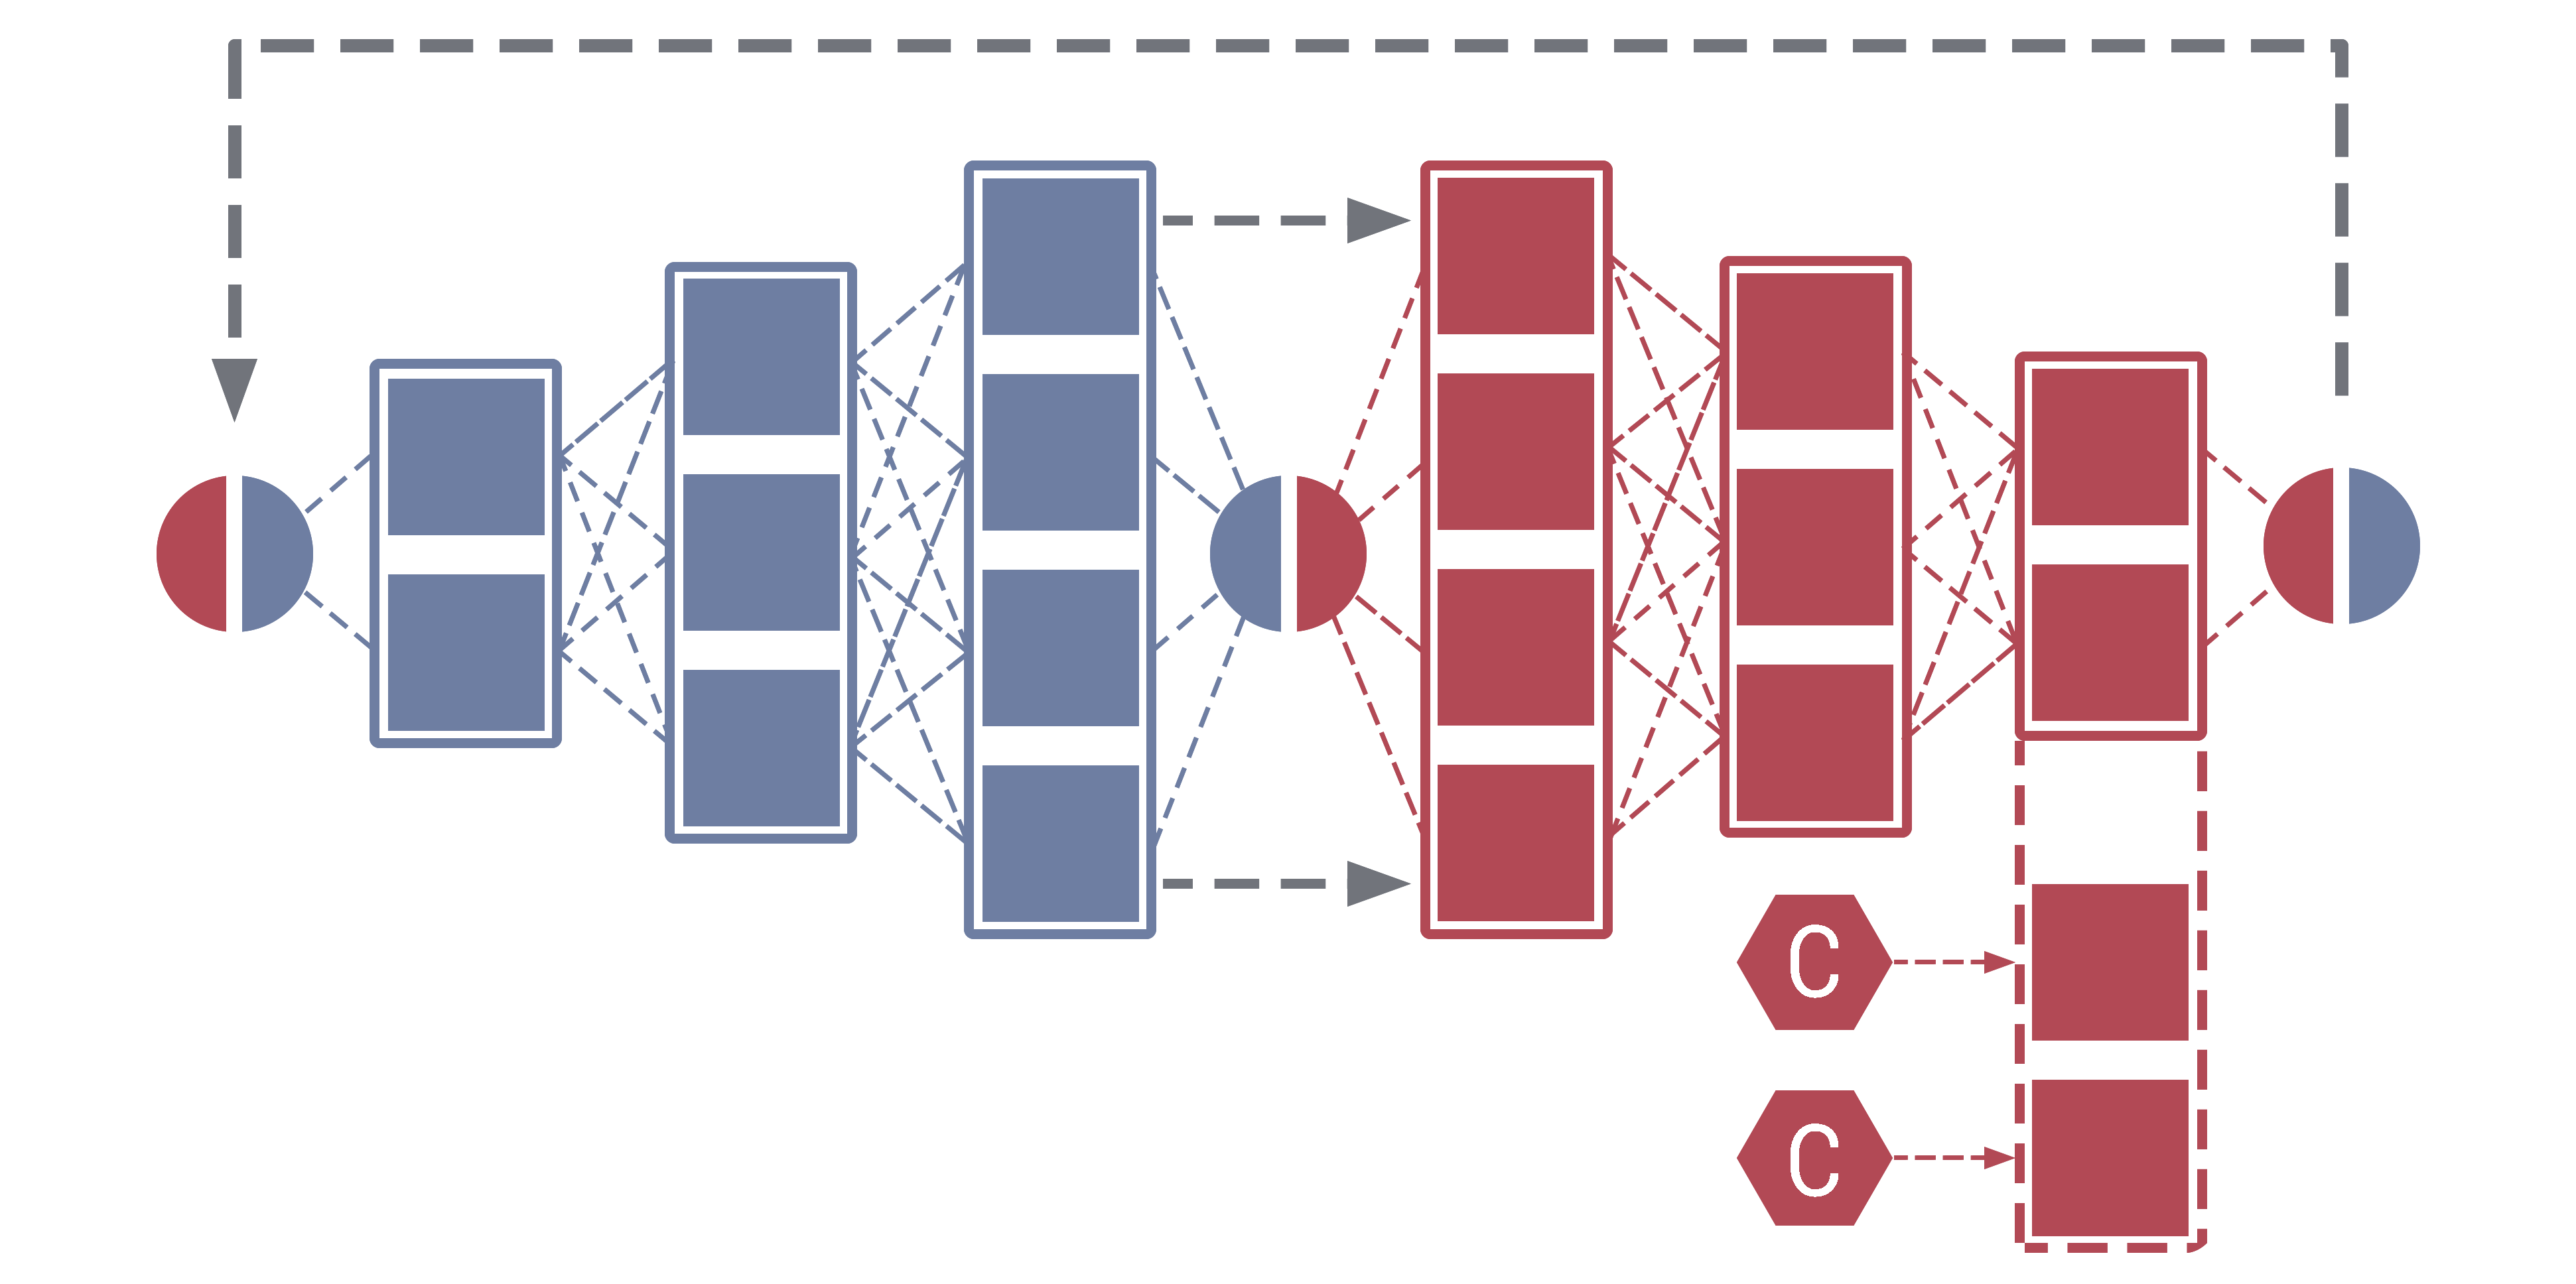
\includegraphics[width=0.7\textwidth]{can20_discr_h32l_schema}
    \caption{Schematic representation of CANs with \textit{can20\_discr\_h32l}. Constraints are introduced in the discriminator (red) in the final hidden layer.}
\end{figure}

\item \textit{can20\_discr\_outl}: discriminator layer with constraints introduced after computing the original output, in an additional final layer.
\begin{enumerate}
    \item $(?, 20, 20, 1) \to (?, 10, 10, 64)$. Type: convolution; filters: 64; kernel size: 5; strides: 2; kernel initializer: Xavier; activation: leaky ReLU ($a = 0.2$).
    \item $(?, 10, 10, 64) \to (?, 5, 5, 128)$. Type: convolution; filters: 128; kernel size: 5; strides: 2; kernel initializer: Xavier; activation: leaky ReLU ($a = 0.2$).
    \item $(?, 5, 5, 128) \stackrel{r}{\to} (?, 3200) \to (?, 1024)$. Type: dense ($1024$ output units); kernel initializer: Xavier; activation: leaky ReLU ($a = 0.2$).
    \item $(?, 1024) \to (?, 1)$. Type: dense ($1$ output units); kernel initializer: Xavier; activation: leaky ReLU ($a = 0.2$).
    \item \textit{if} $|\mathbb{C}| > 0$: $(?, |\mathbb{C}|) \stackrel{c}{\to} (?, 1)$. Type: dense ($1$ output unit); kernel initializer: Xavier; activation: linear.
    \item \textit{if} $|\mathbb{C}| > 0$: $(?, 1) \stackrel{c}{\to} (?, 2) \to (?, 1)$. Type: dense ($1$ output unit); kernel initializer: Xavier; bias initializer: Xavier; activation: linear.
\end{enumerate}

\begin{figure}[ht]
    \centering
    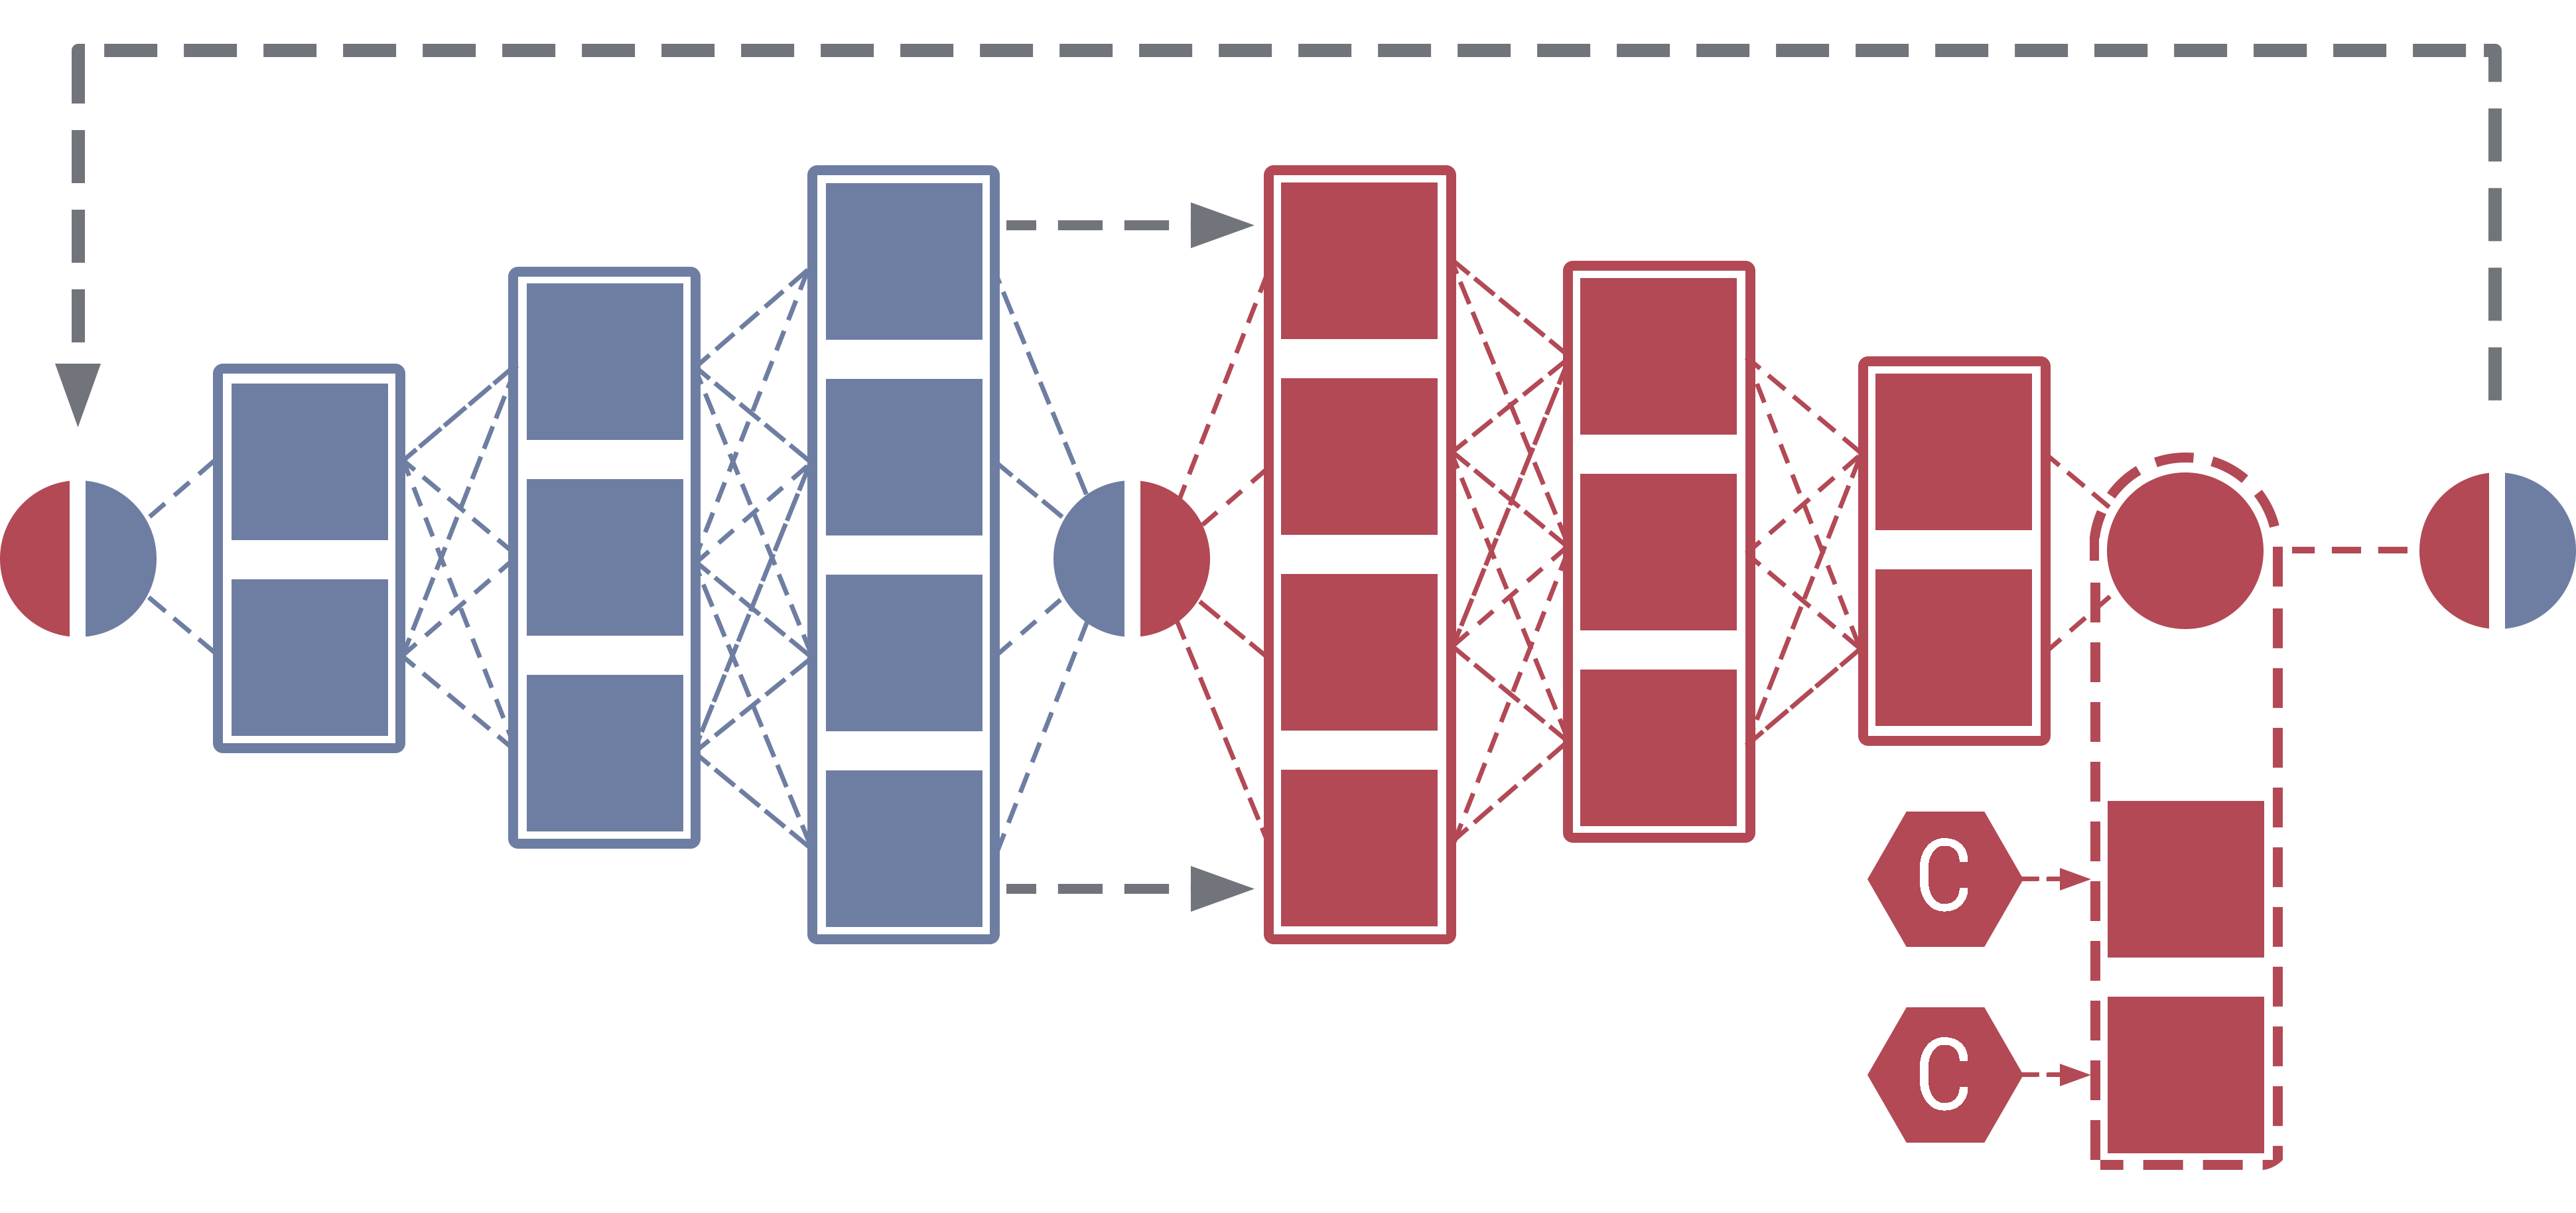
\includegraphics[width=0.7\textwidth]{can20_discr_outl_schema}
    \caption{Schematic representation of CANs with \textit{can20\_discr\_outl}. Constraints are introduced in the discriminator (red) after the final hidden layer.}
\end{figure}

% \item \textit{bgan60\_gen}: generator network originally used for BGANs, adapted for 60x60 pixel data sets. It contains an additional deconvolutional layer (\ref{additional_deconvolution}) to increase model capacity.
% \begin{enumerate}
%     \item $(?, 64) \to (?, 1024)$. Type: dense ($1024$ output units); activation: ReLU; batch normalization. 
%     \item $(?, 1024) \to (?, 3200)$. Type: dense ($3200$ output units); activation: ReLU; batch normalization.
%     \item $(?, 3200) \stackrel{r}{\to} (?, 5, 5, 128) \to (?, 10, 10, 64)$. Type: deconvolution; filters: 64; kernel size: 5; strides: 2; kernel initializer: orthogonal; bias initializer: zeros; activation: ReLU; batch normalization.
%     \item \label{additional_deconvolution} $(?, 10, 10, 64) \to (?, 20, 20, 64)$. Type: deconvolution; filters: 64; kernel size: 5; strides: 2; kernel initializer: orthogonal; bias initializer: zeros; activation: ReLU; batch normalization.
%     \item $(?, 20, 20, 64) \to (?, 60, 60, 1)$. Type: deconvolution; filters: 1; kernel size: 5; strides: 3; kernel initializer: orthogonal; bias initializer: zeros; activation: linear.
%    \end{enumerate}
% 
% \item \textit{can60\_discr\_h32l}: discriminator network originally used for BGANs, adapted for 60x60 pixel data sets. It contains an additional convolutional layer (\ref{additional_convolution}) to increase model capacity.
% \begin{enumerate}
%     \item $(?, 60, 60, 1) \to (?, 30, 30, 64)$. Type: convolution; filters: 64; kernel size: 5; strides: 2; kernel initializer: Xavier; activation: leaky ReLU ($a = 0.2$).
%     \item \label{additional_convolution} $(?, 30, 30, 64) \to (?, 15, 15, 64)$. Type: convolution; filters: 64; kernel size: 5; strides: 2; kernel initializer: Xavier; activation: leaky ReLU ($a = 0.2$).
%     \item $(?, 15, 15, 64) \to (?, 8, 8, 128)$. Type: convolution; filters: 128; kernel size: 5; strides: 2; kernel initializer: Xavier; activation: leaky ReLU ($a = 0.2$).
%     \item $(?, 8, 8, 128) \stackrel{r}{\to} (?, 8192) \to (?, 1024)$. Type: dense ($1024$ output units); kernel initializer: Xavier; activation: leaky ReLU ($a = 0.2$).
%     \item $(?, 1024) \to (?, 32)$. Type: dense ($32$ output units); kernel initializer: Xavier; activation: leaky ReLU ($a = 0.2$).
%     \item \textit{if} $|\mathbb{C}| > 0$: $(?, 32) \stackrel{c}{\to} (?, 32+|\mathbb{C}|)$. Type: dense ($32+|\mathbb{C}|$ output units); kernel initializer: Xavier; bias initializer: Xavier; activation: linear.
%     \item $(?, 32+|\mathbb{C}|) \to (?, 1)$. Type: dense ($1$ output unit); kernel initializer: Xavier; bias initializer: Xavier; activation: linear.
% \end{enumerate}
\end{description}


\section{Penalty functions}

According to the criteria by which data sets \textit{poly20} and \textit{poly20\_pc} have been generated, it is possible to define some constraints on the images. The following is a schematic list, with their corresponding penalty functions and labels.


\begin{description}
\item \textit{smaller\_area}: require the image to not contain less than the expected number of white pixels ($2\times25$). The penalty is proportional to the underestimation.
\begin{enumerate}
\item[] $f(I): min(1, max(0, 2\cdot25 - \sum\limits_{i=1}^{20} \sum\limits_{j=1}^{20} M[i][j]) / (20\cdot20 - 2\cdot25))$
\end{enumerate}

\item \textit{greater\_area}: require the image to not contain more than the expected number of white pixels ($2\times25$). The penalty is proportional to the overestimation.
\begin{enumerate}
\item[] $f(I): min(1, max(0, - 2\cdot25 + \sum\limits_{i=1}^{20} \sum\limits_{j=1}^{20} M[i][j]) / (20\cdot20 - 2\cdot25))$
\end{enumerate}

\item \textit{convex}: require the image to only contain convex shapes. The penalty is proportional to the number of pixels contained in concave zones defined by polygons. Shapes are identified with a breadth-first search in a graph representing the image. Wrong pixels are detected scanning the image by rows, columns and diagonals.
\begin{enumerate}
\item[] $f(I): min(1, (\sum\limits_{i=1}^{20} \sum\limits_{j=1}^{20} M[i][j] \text{ if in concave zone}) / (2\cdot20\cdot20))$
\end{enumerate}

\item \textit{parity\_check\_p\_i}: require the image to correctly set a parity check pixel on the border. The placeholder $p$ can be one of \{rl, rr, ct, cb\} to indicate that the $i\text{-}th$ pixel involves, respectively, a left-half row, a right-half row, a top-half column or a bottom-half column. The penalty assigned is binary: $0$ if the relation \ref{eq:parity_check} is true for the $i\text{-}th$ pixel, $1$ otherwise.

\end{description}


All the penalty functions can be straightforwardly extended to data sets of larger images or with a different number of polygons.

Since experiments have been performed reusing the same sets of penalty functions, additional labels are also provided for them (range notation adopted for conciseness):

\begin{description}
\item \textit{area\_convex}: $\mathbb{C} = \{\textit{smaller\_area, greater\_area, convex}\}$, $|\mathbb{C}| = 3$.

\item \textit{some\_pc}: $\mathbb{C} = \{\textit{smaller\_area, greater\_area, parity\_check\_rl\_1-9, parity\_check\_ct\_1-9}\}$, $|\mathbb{C}| = 20$.

\item \textit{all\_pc}: $\mathbb{C} = \{\textit{smaller\_area, greater\_area, parity\_check\_rl-ct-rr-cb\_1-18}\}$, $|\mathbb{C}| = 74$.
\end{description}



\section{Experiments}

The goal of the first experiment is to compare BGANs and CANs with the simplest data set, \textit{poly20}, and a small set of constraints, \textit{area\_convex}. 
Figures \ref{fig:D_poly20_C_area_convex_N_bgan_can_perfect} and \ref{fig:D_poly20_C_area_convex_N_bgan_can_avg_constraints_satisfaction} show that BGANs are superior to CANs both for the percentage of perfect objects generated and for average constraints satisfaction. The reason is probably related to the constraints involved, that are uninformative and insufficient to better guide the generator in the search space for CANs while introducing additional parameters that unnecessarily burden the training. This evidence justifies the use of the other data set, \textit{poly20\_pc}, and more informative penalty functions.

\begin{figure}[ht]
    \centering
    \begin{minipage}[t]{0.45\textwidth}
        \centering
        \includegraphics[width=\textwidth]{D_poly20_C_area_convex_N_bgan_can_perfect}
        \caption{\\BGANs: \textit{bgan20\_gen} + \textit{bgan20\_discr\_h32l}.\\
        CANs: \textit{bgan20\_gen} + \textit{can20\_discr\_h32l}.}
        \label{fig:D_poly20_C_area_convex_N_bgan_can_perfect}
    \end{minipage}
    \hfill
    \begin{minipage}[t]{0.45\textwidth}
        \centering
        \includegraphics[width=\textwidth]{D_poly20_C_area_convex_N_bgan_can_avg_constraints_satisfaction}
        \caption{\\BGANs: \textit{bgan20\_gen} + \textit{bgan20\_discr\_h32l}.\\
        CANs: \textit{bgan20\_gen} + \textit{can20\_discr\_h32l}.}
        \label{fig:D_poly20_C_area_convex_N_bgan_can_avg_constraints_satisfaction}
    \end{minipage}
\end{figure}


Opposite results are observed when the data distribution to be learnt is harder, such as for \textit{poly20\_pc}. In this case, CANs benefit from the constraints expressed in \textit{some\_pc} and achieve better performance than BGANs, as depicted in figures \ref{fig:D_poly20_pc_C_some_pc_N_bgan_can_perfect} and \ref{fig:D_poly20_pc_C_some_pc_N_bgan_can_avg_constraints_satisfaction}.

\begin{figure}[ht]
    \centering
    \begin{minipage}[t]{0.45\textwidth}
        \centering
        \includegraphics[width=\textwidth]{D_poly20_pc_C_some_pc_N_bgan_can_perfect}
        \caption{\\BGANs: \textit{bgan20\_gen} + \textit{bgan20\_discr\_h32l}.\\
        CANs: \textit{bgan20\_gen} + \textit{can20\_discr\_h32l}.}
        \label{fig:D_poly20_pc_C_some_pc_N_bgan_can_perfect}
    \end{minipage}
    \hfill
    \begin{minipage}[t]{0.45\textwidth}
        \centering
        \includegraphics[width=\textwidth]{D_poly20_pc_C_some_pc_N_bgan_can_avg_constraints_satisfaction}
        \caption{\\BGANs: \textit{bgan20\_gen} + \textit{bgan20\_discr\_h32l}.\\
        CANs: \textit{bgan20\_gen} + \textit{can20\_discr\_h32l}.}
        \label{fig:D_poly20_pc_C_some_pc_N_bgan_can_avg_constraints_satisfaction}
    \end{minipage}
\end{figure}

The differences between the two models are nevertheless small, with the biggest improvement observed in average constraints satisfaction. Figure \ref{fig:D_poly20_pc_C_some_pc_N_bgan_can_avg_constraints_satisfaction_delta} shows that the gap between BGANs and CANs tends to disappear as training continues. This result is reasonable, since BGANs are provided with enough capacity to learn the correct distribution anyway. Nevertheless, it can be considered significative because CANs only require small additional time to be trained, as demonstrated in figure \ref{fig:D_poly20_pc_C_some_pc_N_bgan_can_time}.

\begin{figure}[ht]
    \centering
    \begin{minipage}[t]{0.45\textwidth}
        \centering
        \includegraphics[width=\textwidth]{D_poly20_pc_C_some_pc_N_bgan_can_avg_constraints_satisfaction_delta}
        \caption{\\BGANs: \textit{bgan20\_gen} + \textit{bgan20\_discr\_h32l}.\\
        CANs: \textit{bgan20\_gen} + \textit{can20\_discr\_h32l}.}
        \label{fig:D_poly20_pc_C_some_pc_N_bgan_can_avg_constraints_satisfaction_delta}
    \end{minipage}
    \hfill
    \begin{minipage}[t]{0.45\textwidth}
        \centering
        \includegraphics[width=\textwidth]{D_poly20_pc_C_some_pc_N_bgan_can_time}
        \caption{\\BGANs: \textit{bgan20\_gen} + \textit{bgan20\_discr\_h32l}.\\CANs: \textit{bgan20\_gen} + \textit{can20\_discr\_h32l}.}
        \label{fig:D_poly20_pc_C_some_pc_N_bgan_can_time}
    \end{minipage}
\end{figure}


Some insights can be drawn when comparing two CANs, one using constraints on the last hidden layer and the other on the output layer. Figure \ref{fig:D_poly20_pc_C_some_pc_N_can_canout_perfect} shows how the first architecture is more effective in learning each single constraint in the long term, producing many more perfect objects. On the other side, figure \ref{fig:D_poly20_pc_C_some_pc_N_can_canout_avg_constraints_satisfaction} suggests that modelling the discriminator's output and the constraints as having the same relevance may largely impact the average number of constraints satisfied at the beginning of the training procedure. This trade-off deserves further research in future work.

\begin{figure}[ht]
    \centering
    \begin{minipage}[t]{0.45\textwidth}
        \centering
        \includegraphics[width=\textwidth]{D_poly20_pc_C_some_pc_N_can_canout_perfect}
        \caption{\\CANs: \textit{bgan20\_gen} + \textit{can20\_discr\_h32l}.\\
        CANs\_out: \textit{bgan20\_gen} + \textit{can20\_discr\_outl}.}
        \label{fig:D_poly20_pc_C_some_pc_N_can_canout_perfect}
    \end{minipage}
    \hfill
    \begin{minipage}[t]{0.45\textwidth}
        \centering
        \includegraphics[width=\textwidth]{D_poly20_pc_C_some_pc_N_can_canout_avg_constraints_satisfaction}
        \caption{\\CANs: \textit{bgan20\_gen} + \textit{can20\_discr\_h32l}.\\
        CANs\_out: \textit{bgan20\_gen} + \textit{can20\_discr\_outl}.}
        \label{fig:D_poly20_pc_C_some_pc_N_can_canout_avg_constraints_satisfaction}
    \end{minipage}
\end{figure}


In all the experiments presented so far using the set of constraints \textit{some\_pc} it is evident that networks achieve excellent performances in satisfying each constraint on average ($95\%+$), but not in generating perfect objects (${\sim}65\%$). The same experiments have also been conducted using a double amount of training epochs. Figure \ref{fig:D_poly20_pc_C_some_pc_N_bgan_can_bganlong_canlong_perfect} shows that, on longer runs, not only the number of perfect objects increases over epochs, but the gap between BGANs and CANs is also preserved.


The ratio behind using only a subset of available parity checks as constraints is that network capable of satisfying some of them should in principle be able to satisfy all of them. This hypothesis is tested by using the complete set of constraints, \textit{all\_pc}.

Figure \ref{fig:D_poly20_pc_C_all_pc_N_bgan_can_perfect} reports the results achieved with a set up equal to that of figure \ref{fig:D_poly20_pc_C_some_pc_N_bgan_can_perfect} but for the usage of the extended constraints set. As expected, both the models now require more training epochs before being able to generate perfect objects (at least $50$). A more interesting observation regards the same performance measured at the end of the training algorithm. It is possible to notice that CANs succeed in generating objects satisfying the two set of constraints with approximately the same probability, while BGANs suffer a great performance loss. The result is better highlighted in figure \ref{fig:D_poly20_pc_C_all_pc_N_bgan_can_perfect_delta}, where a remarkable gap of $16\%$ can be observed between the two architectures at the hundredth epoch.

\begin{figure}[ht]
    \centering
    \begin{minipage}[t]{0.45\textwidth}
        \centering
        \includegraphics[width=\textwidth]{D_poly20_pc_C_some_pc_N_bgan_can_bganlong_canlong_perfect}
        \caption{\\BGANs: \textit{bgan20\_gen} + \textit{bgan20\_discr\_h32l}.\\
        CANs: \textit{bgan20\_gen} + \textit{can20\_discr\_h32l}.\\
        BGANs\_long = BGANs\\
        CANs\_long = CANs.}
        \label{fig:D_poly20_pc_C_some_pc_N_bgan_can_bganlong_canlong_perfect}
    \end{minipage}
    \hfill
    \begin{minipage}[t]{0.45\textwidth}
        \centering
        \includegraphics[width=\textwidth]{D_poly20_pc_C_all_pc_N_bgan_can_perfect}
        \caption{\\BGANs: \textit{bgan20\_gen} + \textit{bgan20\_discr\_h32l}.\\
        CANs: \textit{bgan20\_gen} + \textit{can20\_discr\_h32l}.}
        \label{fig:D_poly20_pc_C_all_pc_N_bgan_can_perfect}
    \end{minipage}
\end{figure}

It is worth noting that, due to the kind of constraints involved and to the multi-core implementation, the difference in execution times remains small, as reported in figure \ref{fig:D_poly20_pc_C_all_pc_N_bgan_can_time}. This proves that the model is able to scale and to learn how to satisfy constraints in polynomial-time if penalty functions can be evaluated in polynomial-time as well. Results regarding average constraints satisfaction are similar to the previous ones and thus omitted.

\begin{figure}[ht]
    \centering
    \begin{minipage}[t]{0.45\textwidth}
        \centering
        \includegraphics[width=\textwidth]{D_poly20_pc_C_all_pc_N_bgan_can_perfect_delta}
        \caption{\\BGANs: \textit{bgan20\_gen} + \textit{bgan20\_discr\_h32l}.\\
        CANs: \textit{bgan20\_gen} + \textit{can20\_discr\_h32l}.}
        \label{fig:D_poly20_pc_C_all_pc_N_bgan_can_perfect_delta}
    \end{minipage}
    \hfill
    \begin{minipage}[t]{0.45\textwidth}
        \centering
        \includegraphics[width=\textwidth]{D_poly20_pc_C_all_pc_N_bgan_can_time}
        \caption{\\BGANs: \textit{bgan20\_gen} + \textit{bgan20\_discr\_h32l}.\\
        CANs: \textit{bgan20\_gen} + \textit{can20\_discr\_h32l}.}
        \label{fig:D_poly20_pc_C_all_pc_N_bgan_can_time}
    \end{minipage}
\end{figure}

% \todor{Another important aspect that must still be evaluated involves the moment in which constraints should be introduced in the training procedure, as discussed in \ref{subsec:constraints_timing}. Many different preliminary experiments have been performed in order to detect automatically the optimal epoch, relying on statistics progressively collected on a validation set. No significant evidence arises from these experiments, so they are omitted for brevity. For the sake of completeness, however, figures \ref{fig:D_poly20_pc_C_all_pc_N_bgan_can_canout_candelay_avg_constraints_satisfaction} and \ref{fig:D_poly20_pc_C_all_pc_N_bgan_can_canout_candelay_perfect} report the results obtained in the same configuration of the previous experiment on other architectures. It is clear that dynamically introducing constraints in a later training phase (e.g. at epoch $100$) does not help the generator. The idea to first let the model learn global properties of objects and then refine its knowledge by introducing constraints thus seems not effective. An informal explanation may be that the generator has already learnt how to model $p_{data}$ and introducing constraints in the adversarial training only causes an imbalance that would force him to forget and re-learn. Additional experiments may explore this research question.}{Abbiamo troppi pochi risultati per fare queste considerazioni, io toglierei discussione e grafici}
% 
% \begin{figure}[ht]
%     \centering
%     \begin{minipage}[t]{0.45\textwidth}
%         \centering
%         \includegraphics[width=\textwidth]{D_poly20_pc_C_all_pc_N_bgan_can_canout_candelay_avg_constraints_satisfaction}
%         \caption{\\BGANs: \textit{bgan20\_gen} + \textit{bgan20\_discr\_h32l}.\\
%         CANs: \textit{bgan20\_gen} + \textit{can20\_discr\_h32l}.\\
%         CANs\_out: \textit{bgan20\_gen} + \textit{can20\_discr\_outl}.\\
%         CANs\_e100 = CANs.\\
%         Constraints are used in CANs\_e100 only from epoch $100$.}
%         \label{fig:D_poly20_pc_C_all_pc_N_bgan_can_canout_candelay_avg_constraints_satisfaction}
%     \end{minipage}
%     \hfill
%     \begin{minipage}[t]{0.45\textwidth}
%         \centering
%         \includegraphics[width=\textwidth]{D_poly20_pc_C_all_pc_N_bgan_can_canout_candelay_perfect}
%         \caption{\\BGANs: \textit{bgan20\_gen} + \textit{bgan20\_discr\_h32l}.\\
%         CANs: \textit{bgan20\_gen} + \textit{can20\_discr\_h32l}.\\
%         CANs\_out: \textit{bgan20\_gen} + \textit{can20\_discr\_outl}.\\
%         CANs\_e100 = CANs.\\
%         Constraints are used in CANs\_e100 only from epoch $100$.}
%         \label{fig:D_poly20_pc_C_all_pc_N_bgan_can_canout_candelay_perfect}
%     \end{minipage}
% \end{figure}


In all the results presented so far CANs appear to improve the BGANs baseline when they have early access to constraints and when penalty functions can be effectively used to guide the network in the search space. However, none of the experiments has evaluated the impact of the size of the data set. To estimate the impact of the number of training examples on the model performance a new smaller data set, \textit{poly20\_pc\_small}, is used. It contains one half of the training examples of \textit{poly20\_pc}, thus being composed of $13,568$ images ($9,472$ for training, $4,096$ for testing).

Results on the same experimental set up are reported in figures \ref{fig:D_poly20_pc_small_C_all_pc_N_bgan_can_avg_constraints_satisfaction} and \ref{fig:D_poly20_pc_small_C_all_pc_N_bgan_can_perfect}. With the smaller data set the gap between CANs and BGANs increases considerably according both to average constraints satisfaction and to the number of perfect objects generated. In this configuration constraints are the most effective and CANs score an improvement superior to $20\%$ to their counterpart, as highlighted in figure  \ref{fig:D_poly20_pc_small_C_all_pc_N_bgan_can_perfect_delta}.

\begin{figure}[ht]
    \centering
    \begin{minipage}[t]{0.45\textwidth}
        \centering
        \includegraphics[width=\textwidth]{D_poly20_pc_small_C_all_pc_N_bgan_can_avg_constraints_satisfaction}
        \caption{\\BGANs: \textit{bgan20\_gen} + \textit{bgan20\_discr\_h32l}.\\
        CANs: \textit{bgan20\_gen} + \textit{can20\_discr\_h32l}.}
        \label{fig:D_poly20_pc_small_C_all_pc_N_bgan_can_avg_constraints_satisfaction}
    \end{minipage}
    \hfill
    \begin{minipage}[t]{0.45\textwidth}
        \centering
        \includegraphics[width=\textwidth]{D_poly20_pc_small_C_all_pc_N_bgan_can_perfect}
        \caption{\\BGANs: \textit{bgan20\_gen} + \textit{bgan20\_discr\_h32l}.\\
        CANs: \textit{bgan20\_gen} + \textit{can20\_discr\_h32l}.}
        \label{fig:D_poly20_pc_small_C_all_pc_N_bgan_can_perfect}
    \end{minipage}
\end{figure}

\begin{figure}[ht]
    \centering
    \begin{minipage}[t]{0.45\textwidth}
        \centering
        \includegraphics[width=\textwidth]{D_poly20_pc_small_C_all_pc_N_bgan_can_perfect_delta}
        \caption{\\BGANs: \textit{bgan20\_gen} + \textit{bgan20\_discr\_h32l}.\\
        CANs: \textit{bgan20\_gen} + \textit{can20\_discr\_h32l}.}
        \label{fig:D_poly20_pc_small_C_all_pc_N_bgan_can_perfect_delta}
    \end{minipage}
    \hfill
    \begin{minipage}[t]{0.45\textwidth}
        \centering
        \includegraphics[width=\textwidth]{D_poly20_pc_small_C_all_pc_N_bgan_can_avg_constraints_satisfaction_delta}
        \caption{\\BGANs: \textit{bgan20\_gen} + \textit{bgan20\_discr\_h32l}.\\
        CANs: \textit{bgan20\_gen} + \textit{can20\_discr\_h32l}.}
        \label{fig:D_poly20_pc_small_C_all_pc_N_bgan_can_avg_constraints_satisfaction_delta}
    \end{minipage}
\end{figure}


\begin{figure}[ht]
    \centering
    \begin{minipage}{0.32\textwidth}
        \centering
        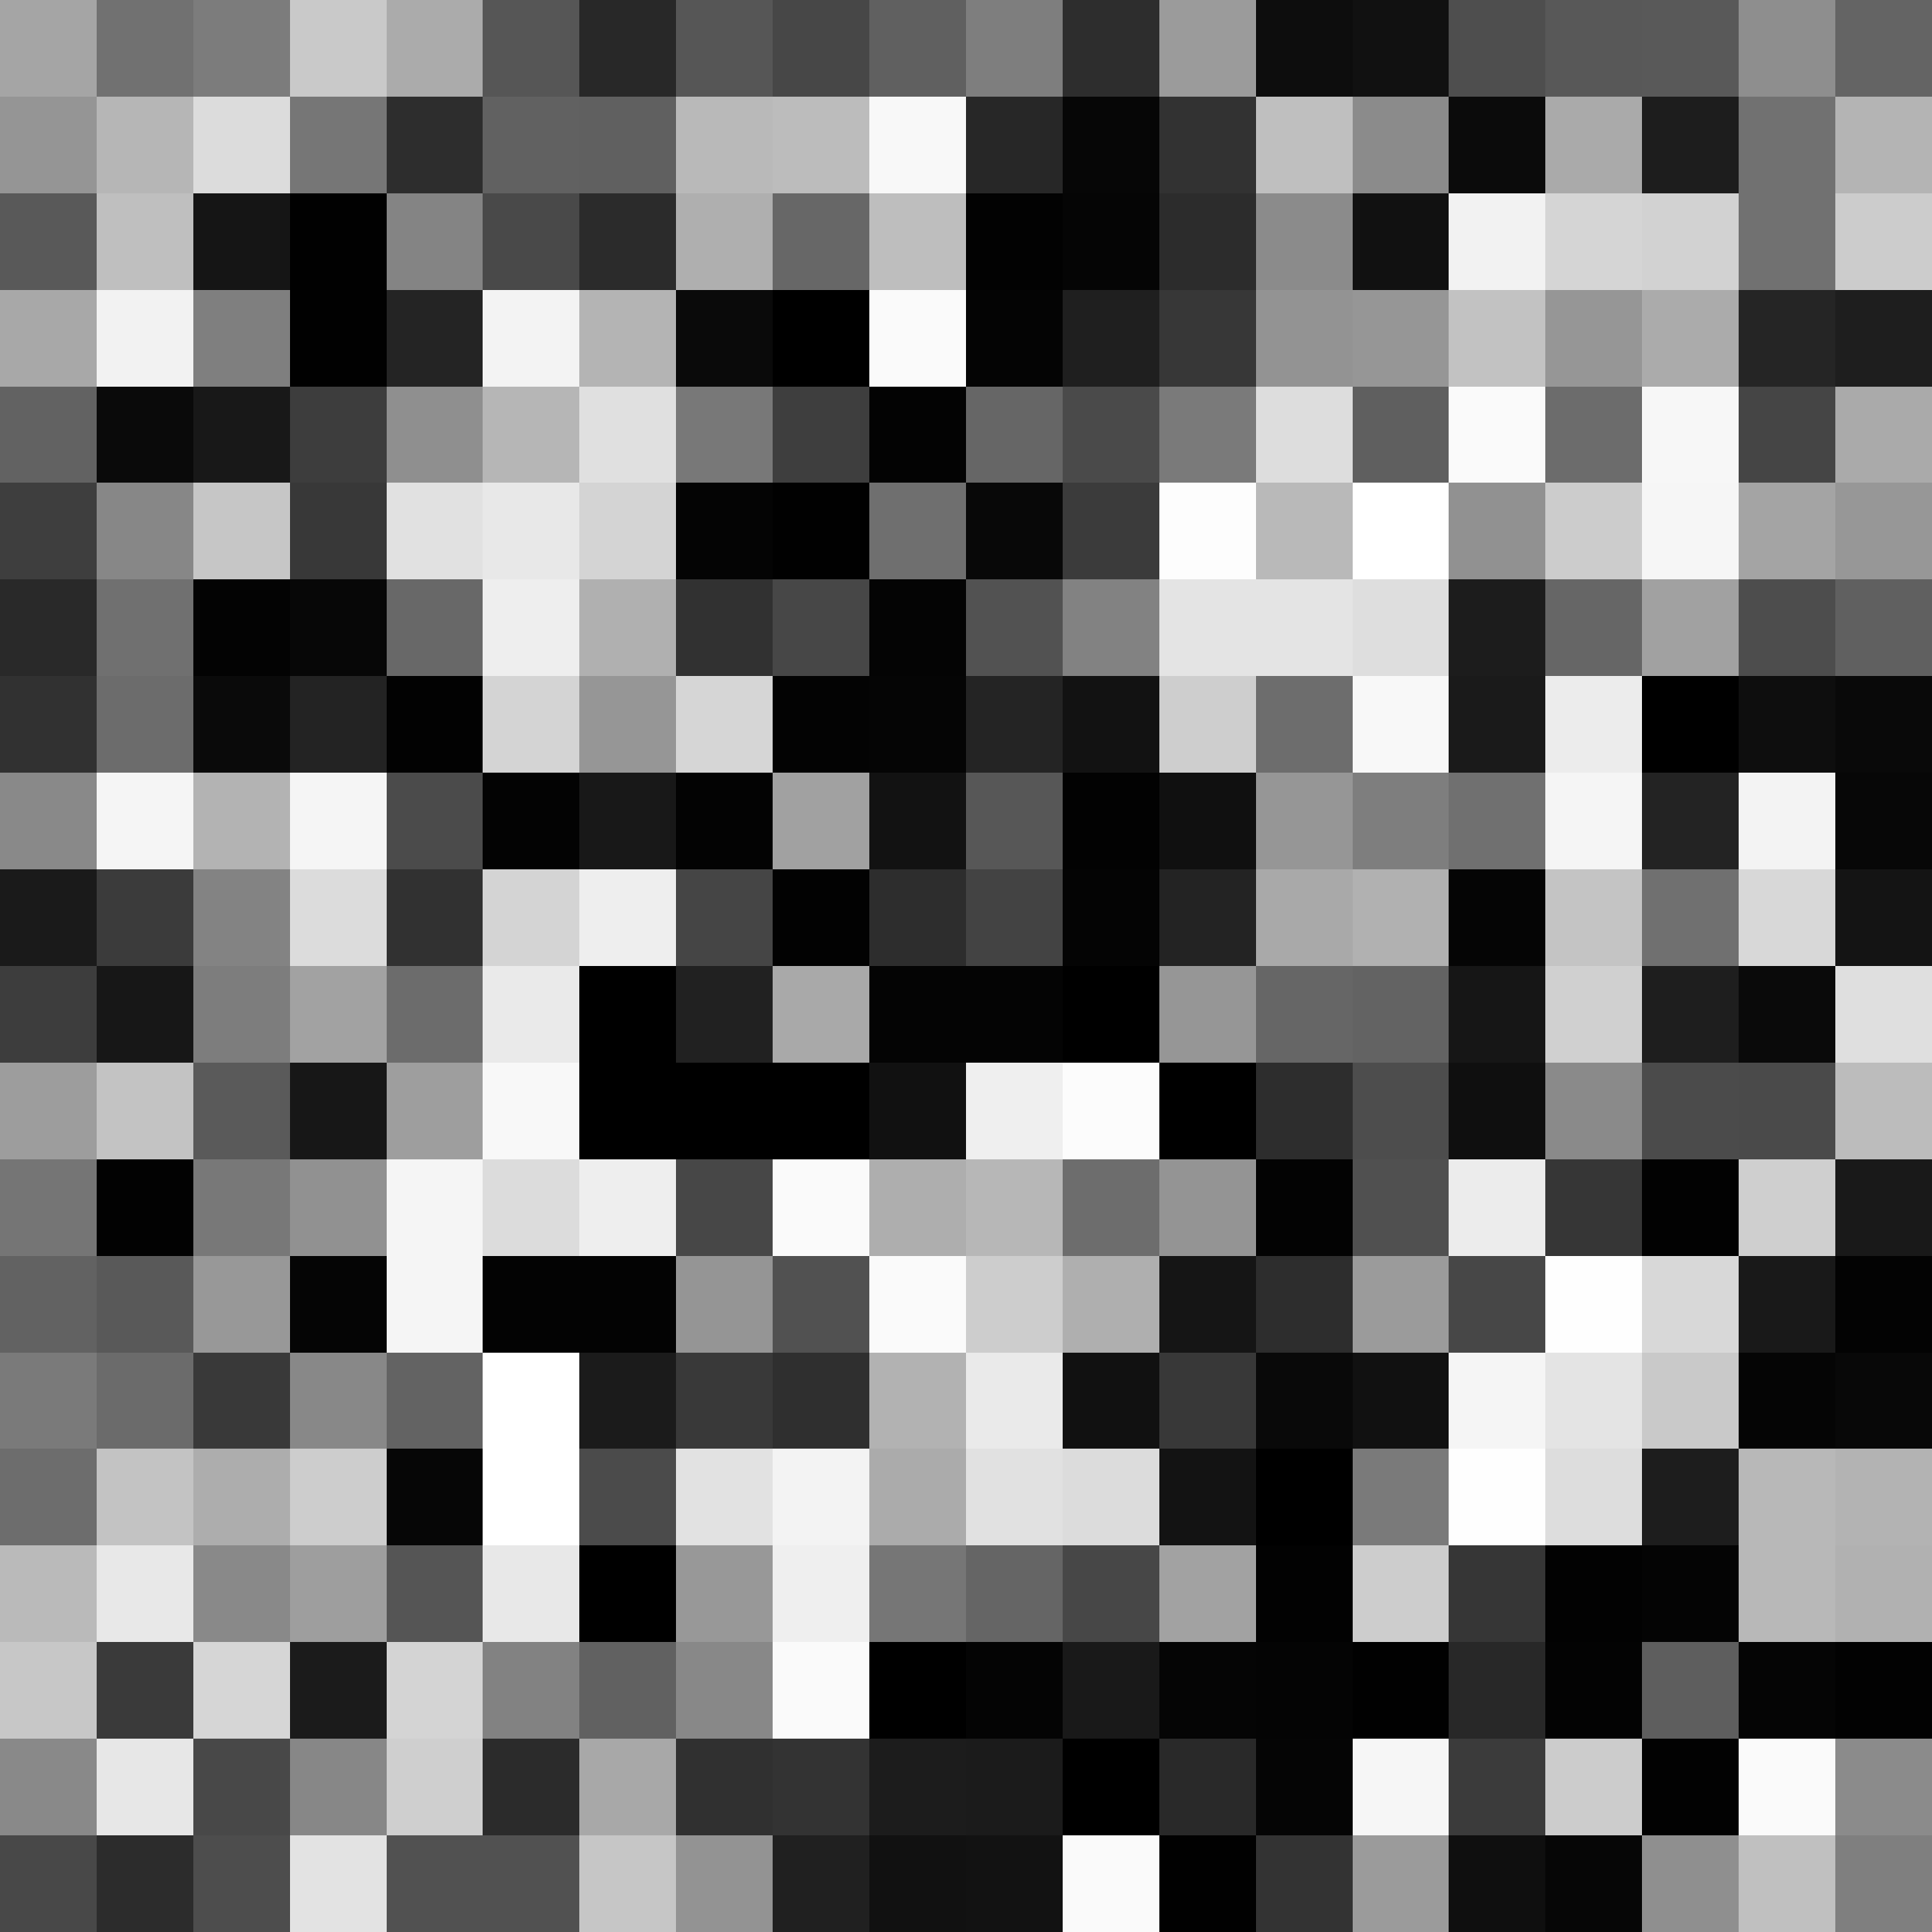
\includegraphics[width=\textwidth]{training_1}
    \end{minipage}
    \begin{minipage}{0.32\textwidth}
        \centering
        
\includegraphics[width=\textwidth]{training_2}
    \end{minipage}
    \begin{minipage}{0.32\textwidth}
        \centering
        
\includegraphics[width=\textwidth]{training_3}
    \end{minipage}
    \vspace{0.3cm}
    \begin{minipage}{0.32\textwidth}
        \centering
        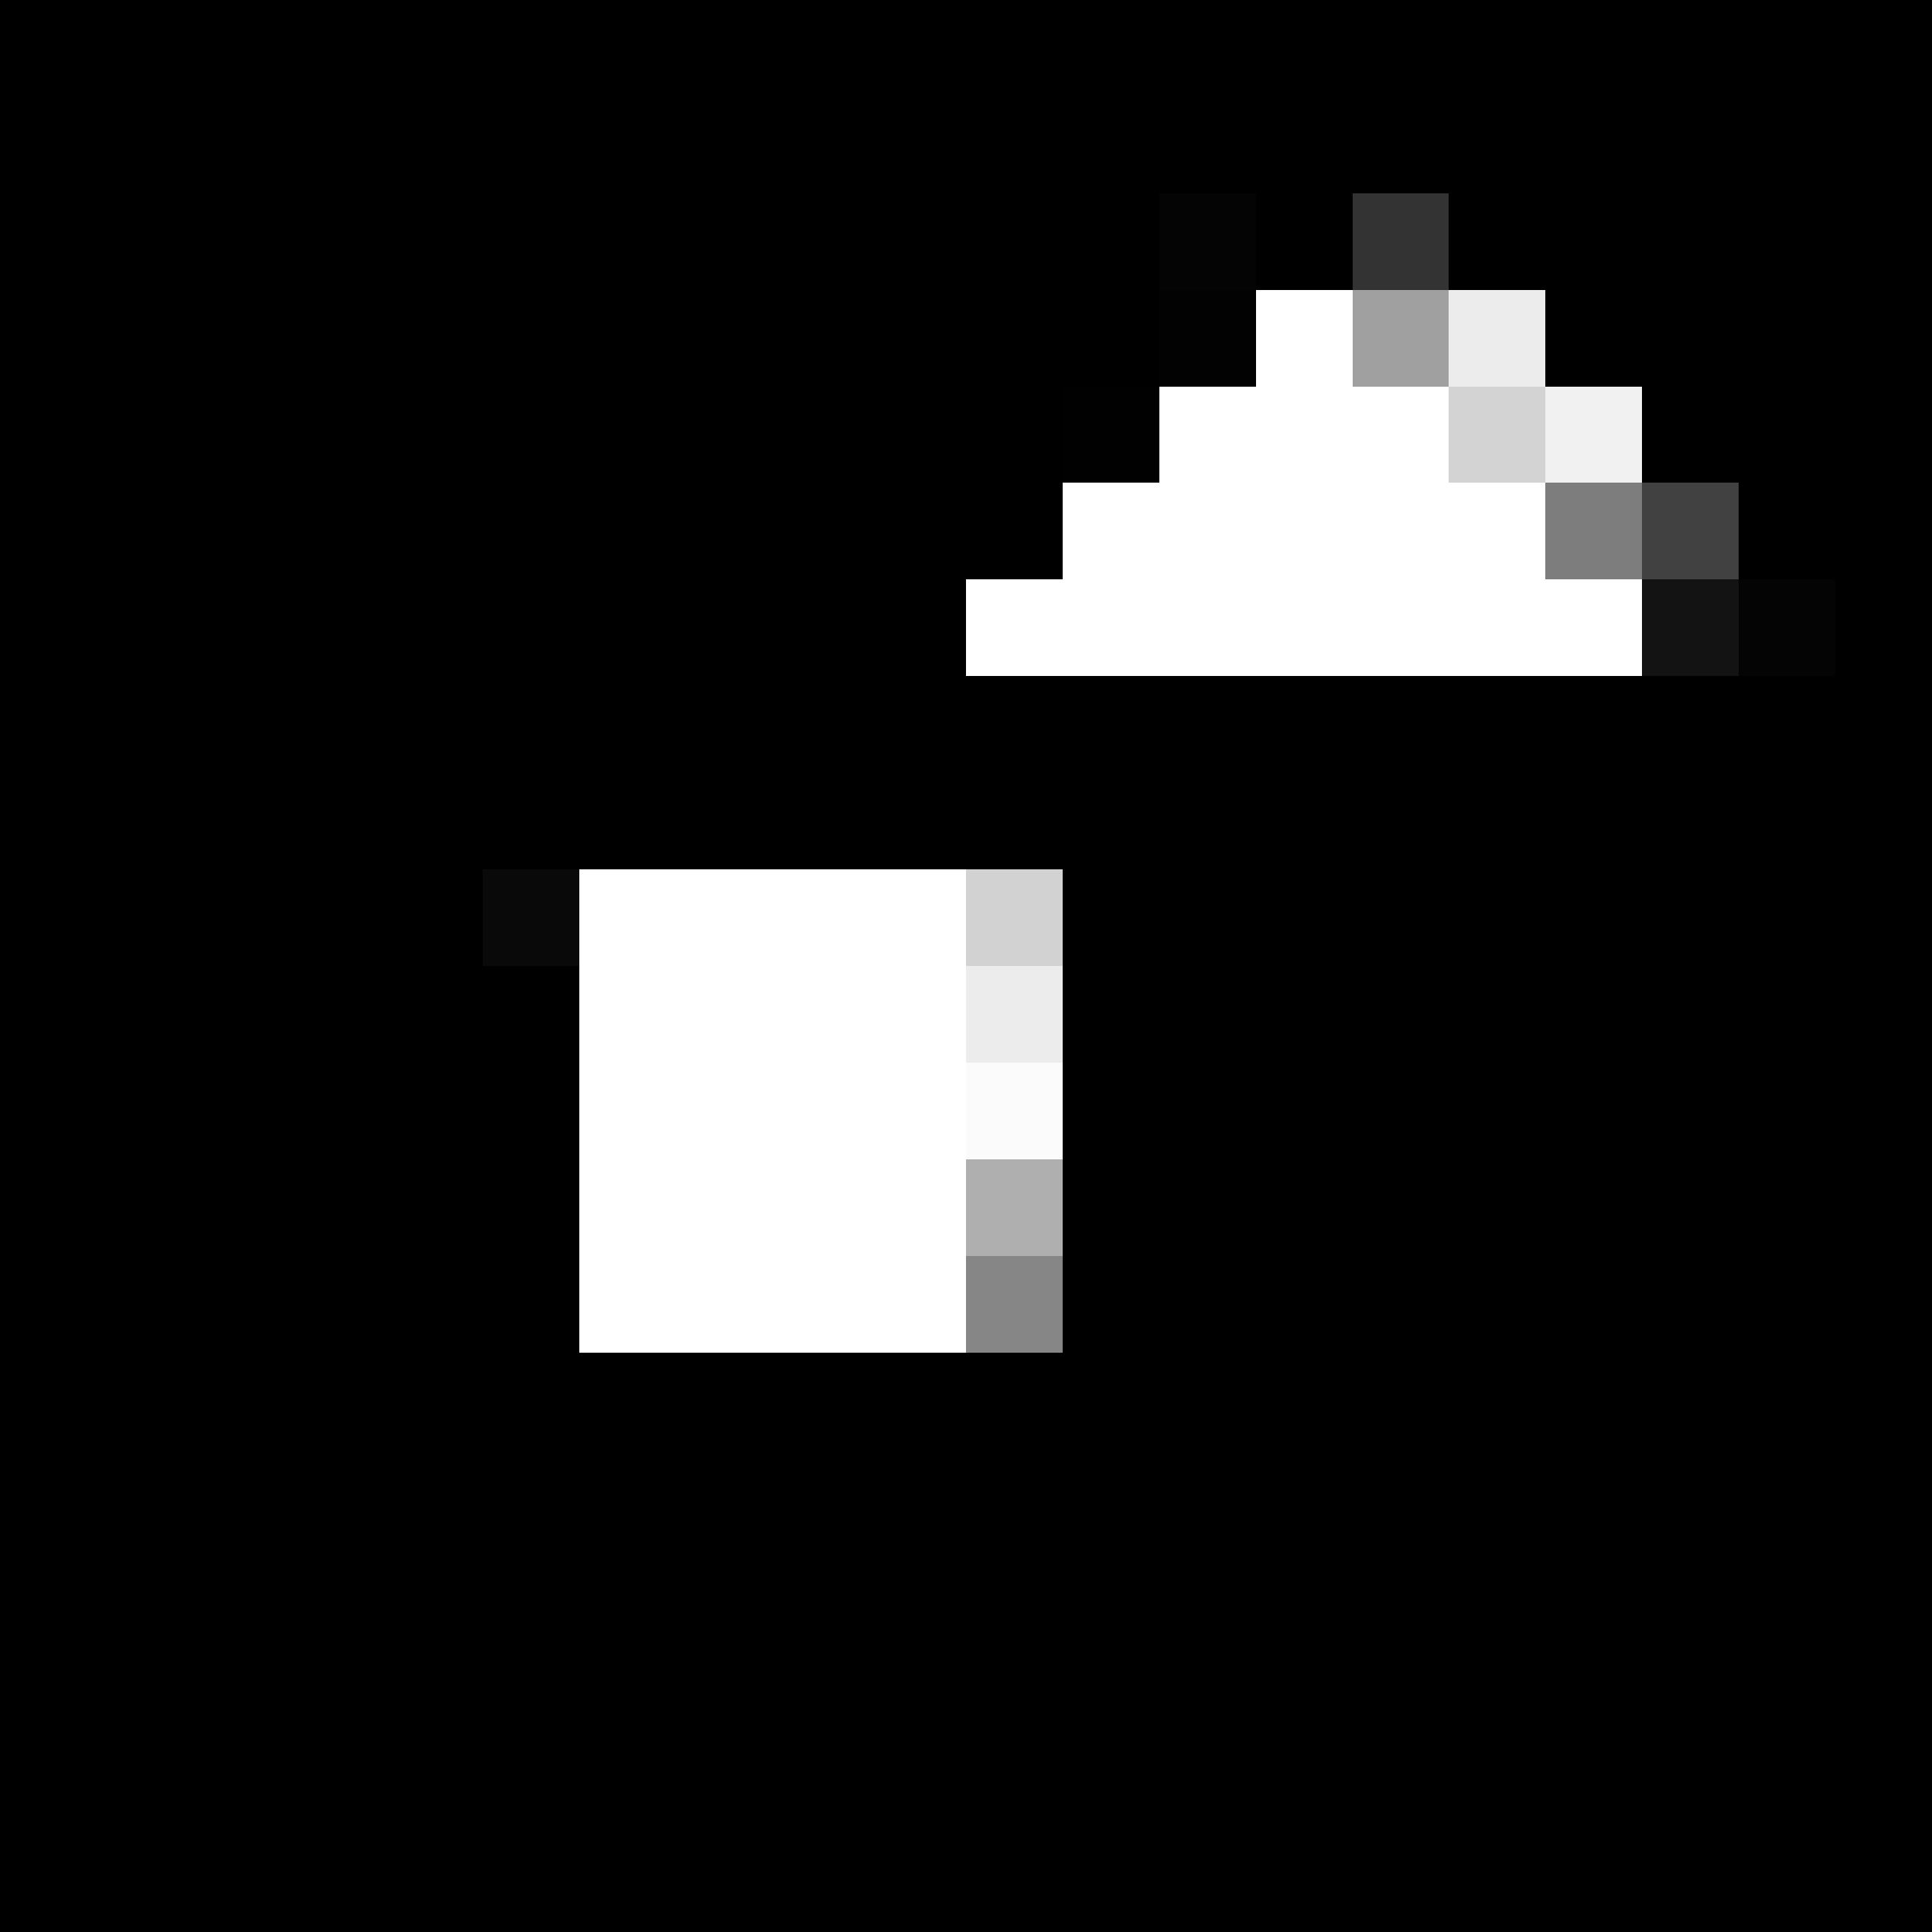
\includegraphics[width=\textwidth]{training_4}
    \end{minipage}
    \begin{minipage}{0.32\textwidth}
        \centering
        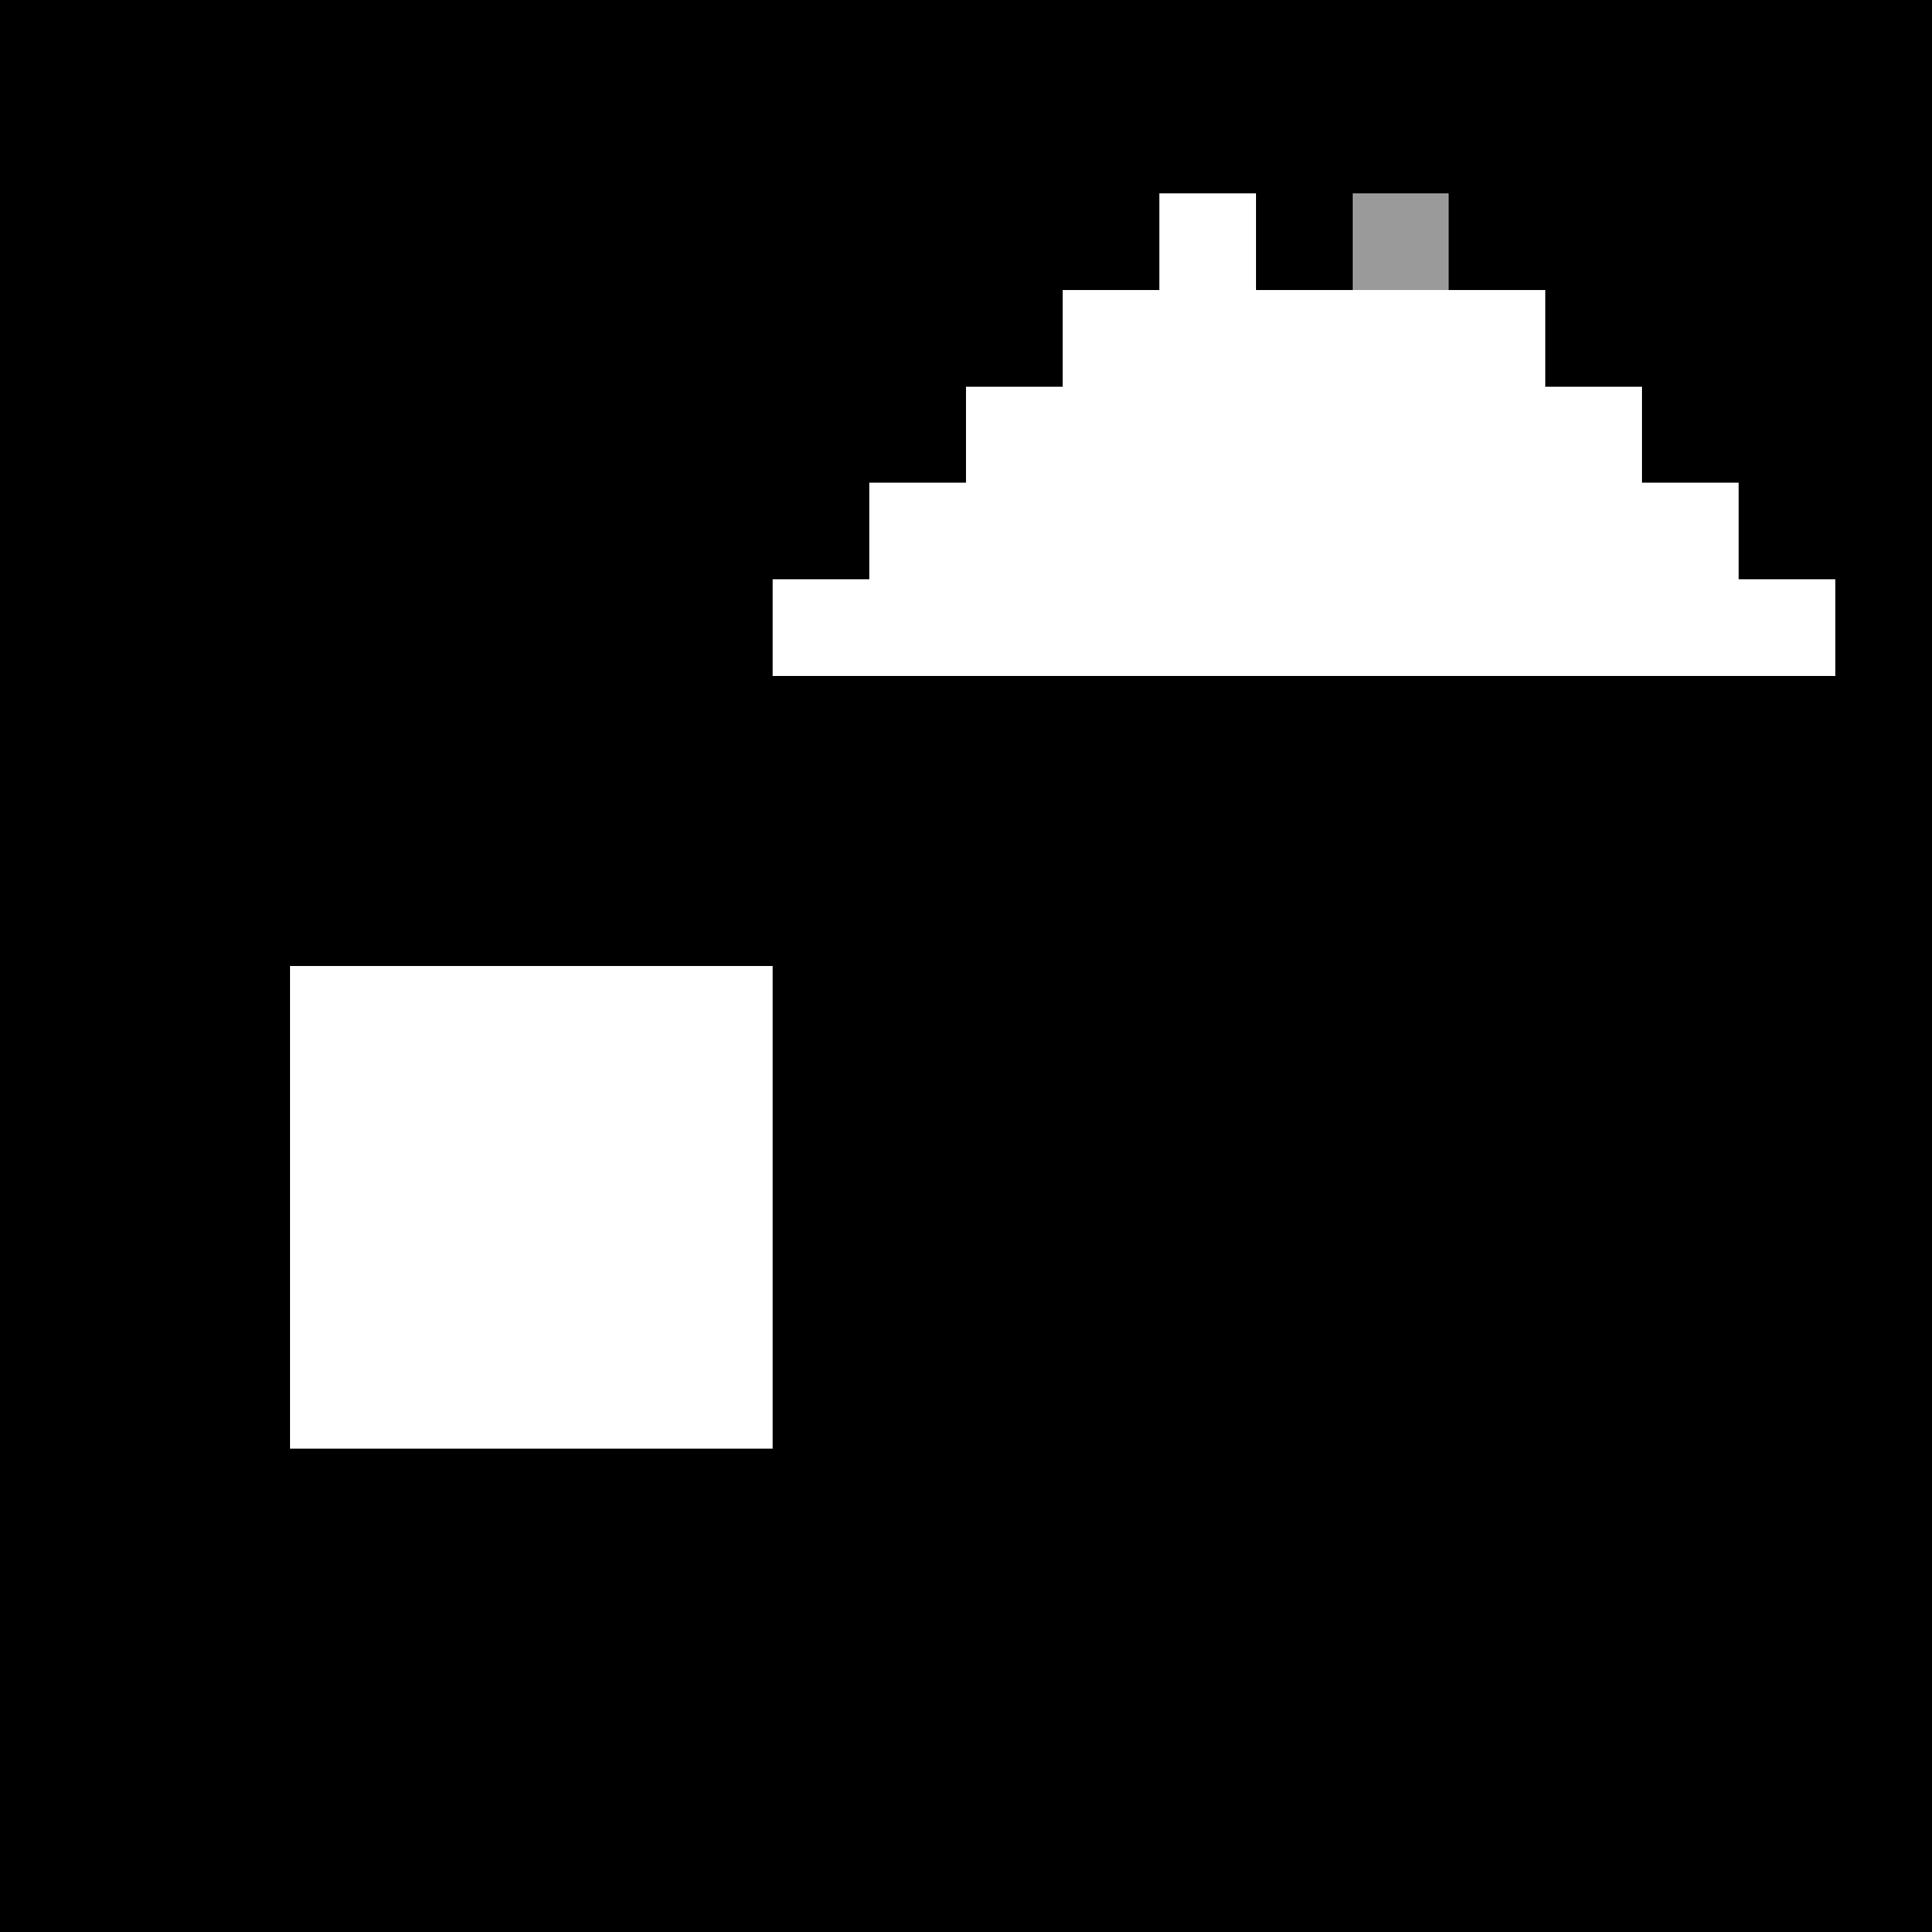
\includegraphics[width=\textwidth]{training_5}
    \end{minipage}
    \begin{minipage}{0.32\textwidth}
        \centering
        
\includegraphics[width=\textwidth]{training_6}
    \end{minipage}
    \caption{Samples drawn at different epochs from the generator trained on \textit{poly20} (zoom).}
\end{figure}


\begin{figure}[ht]
    \centering
    \begin{minipage}{0.32\textwidth}
        \centering
        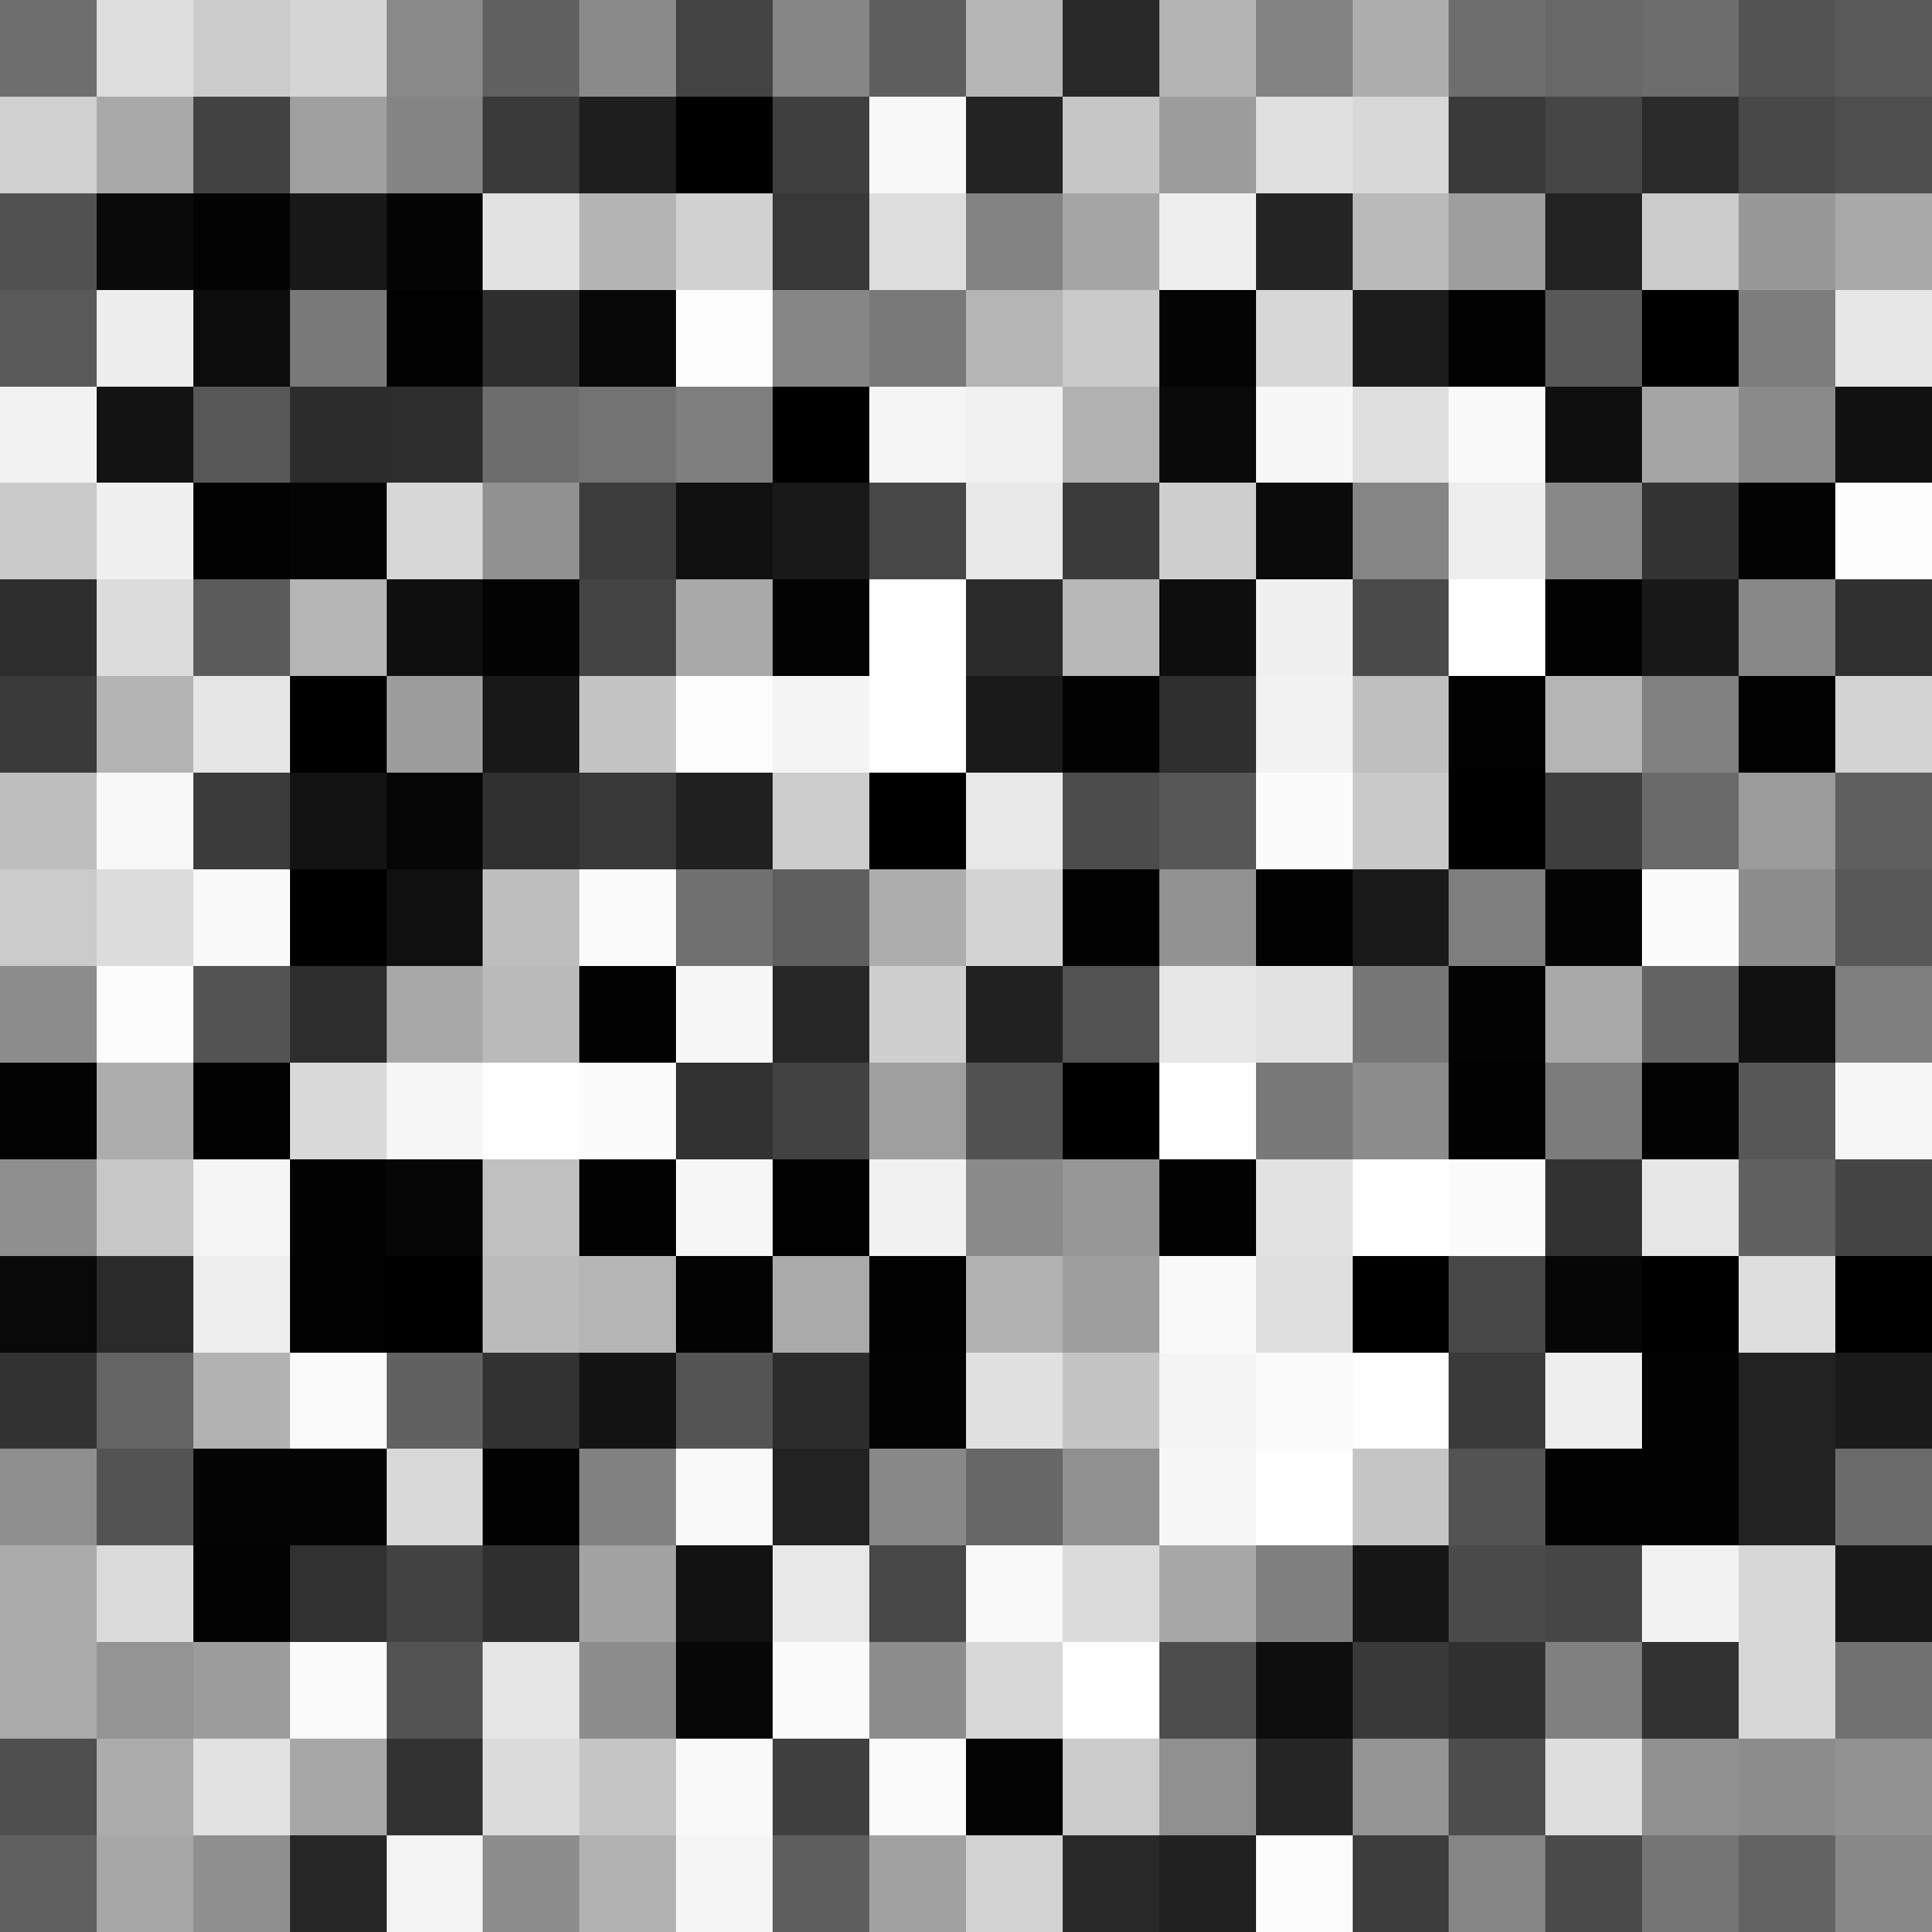
\includegraphics[width=\textwidth]{training_pc_1}
    \end{minipage}
    \begin{minipage}{0.32\textwidth}
        \centering
        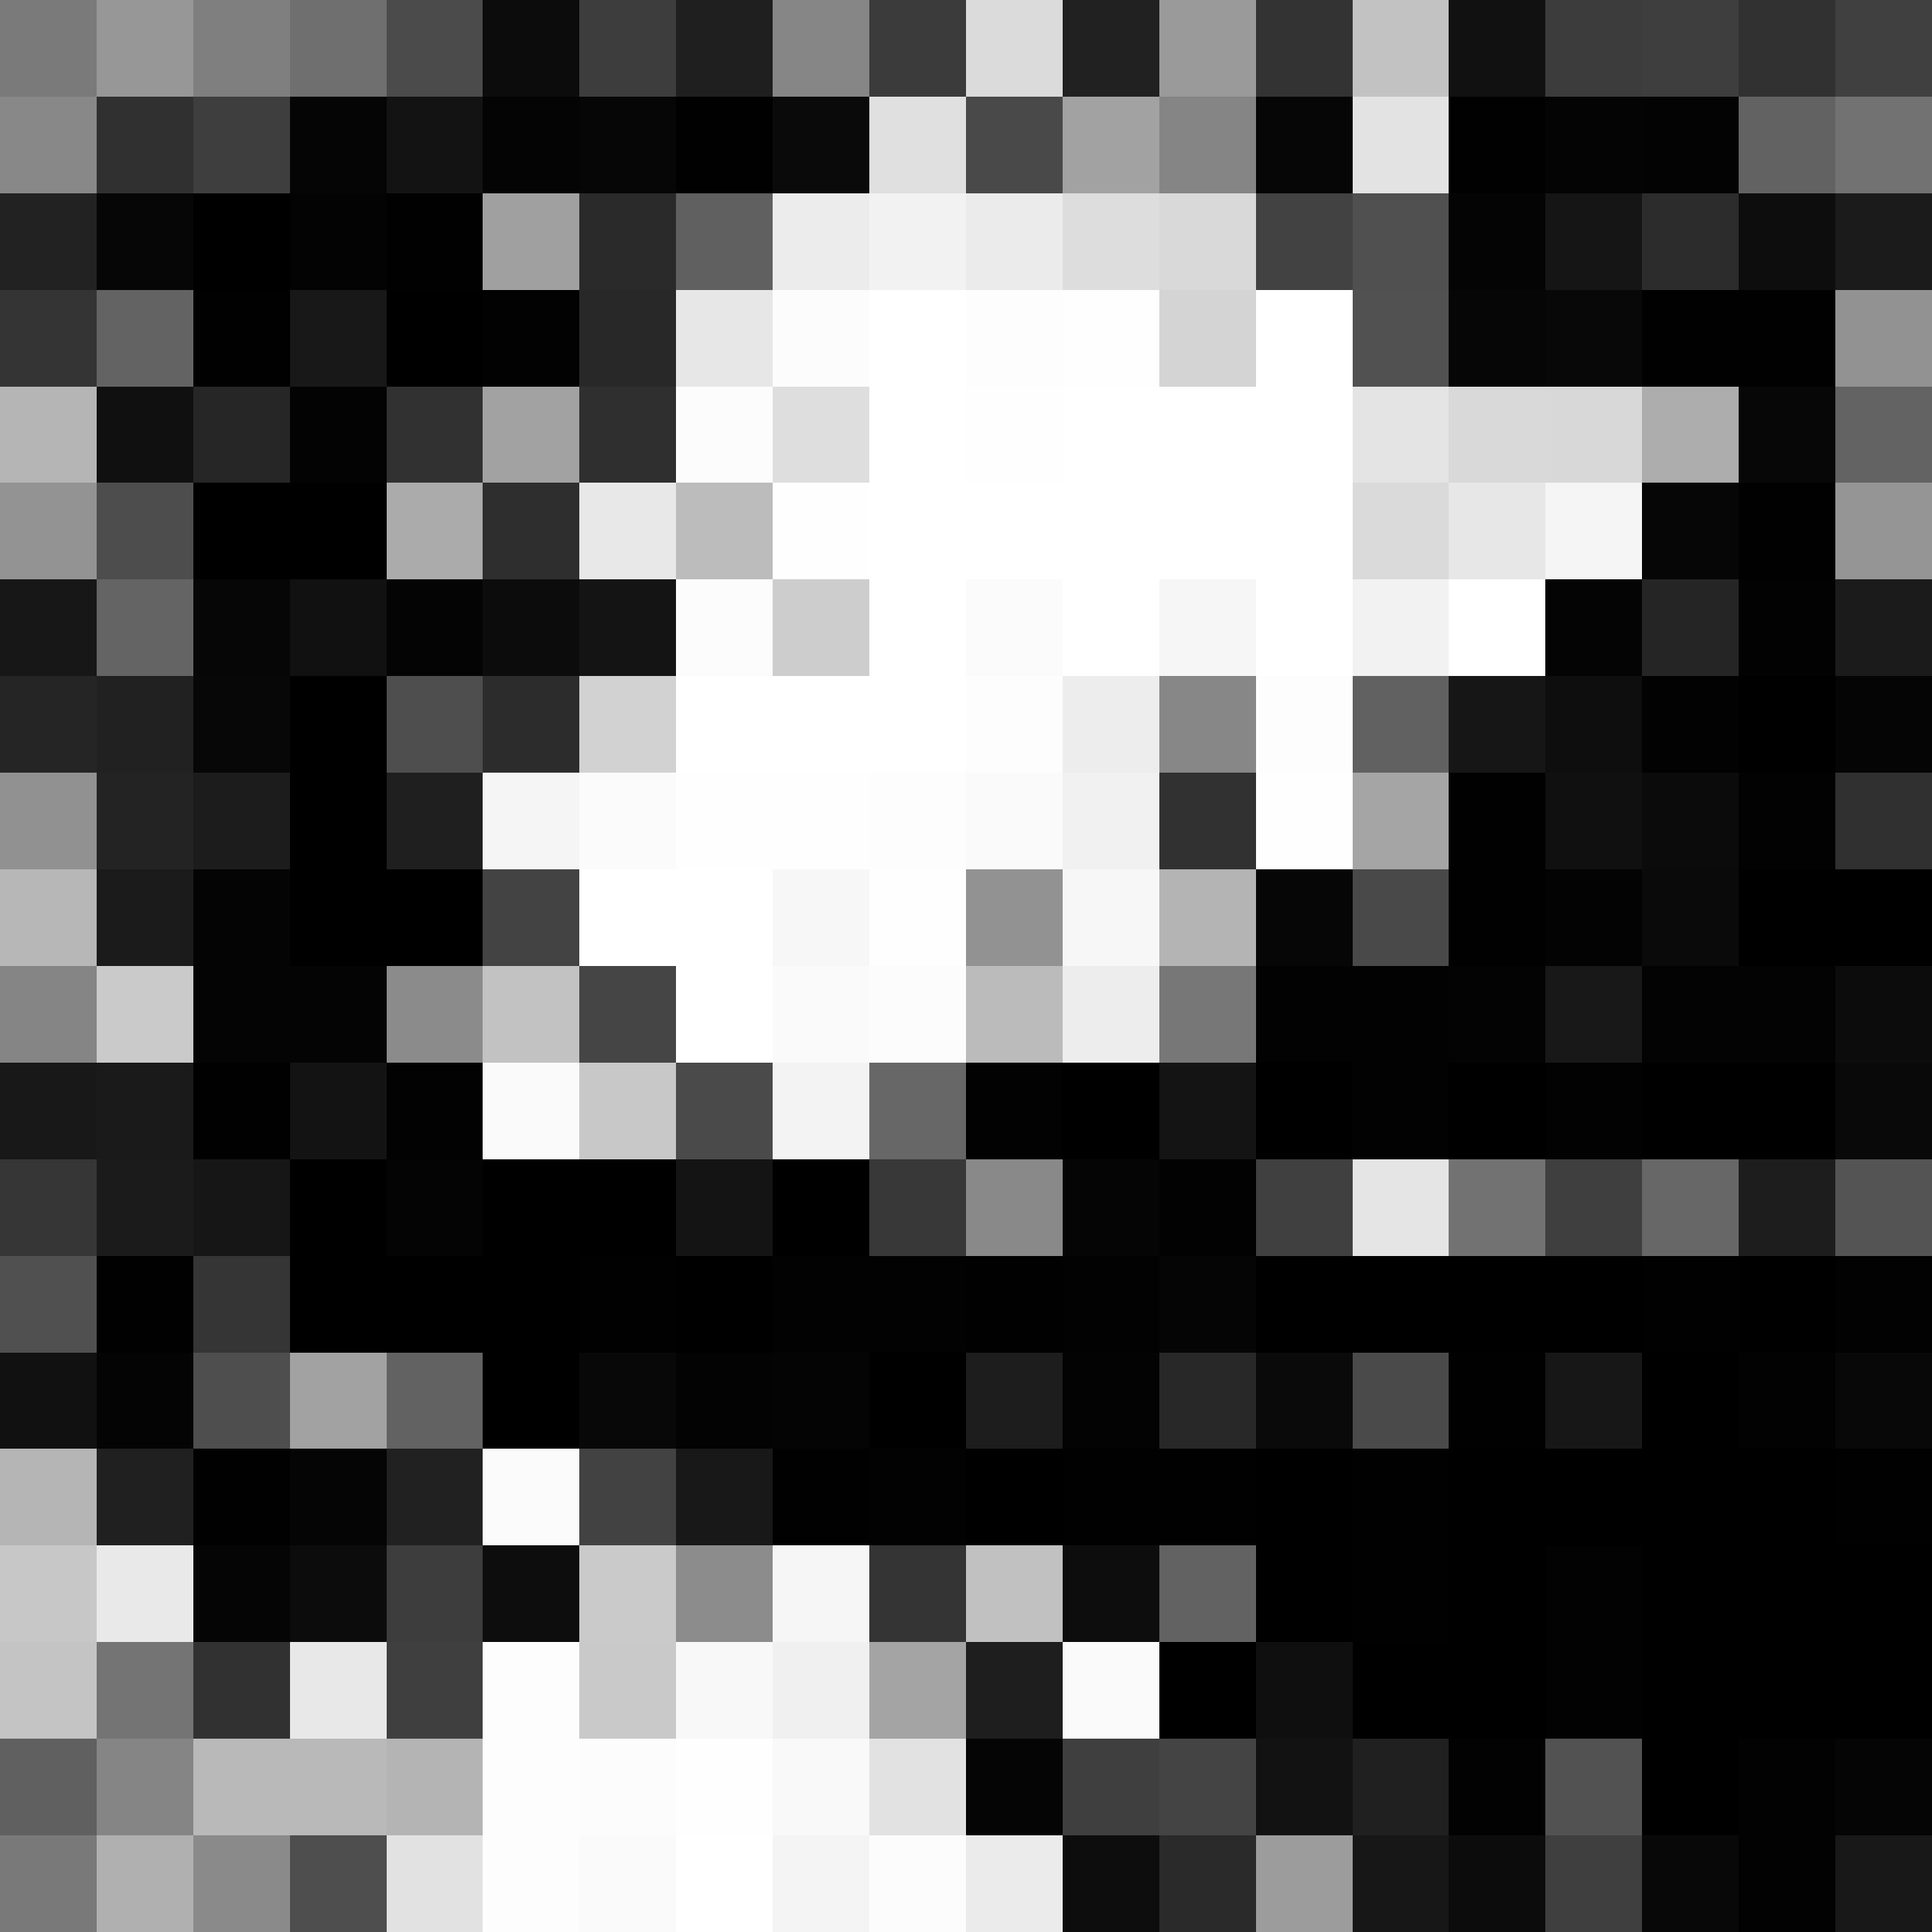
\includegraphics[width=\textwidth]{training_pc_2}
    \end{minipage}
    \begin{minipage}{0.32\textwidth}
        \centering
        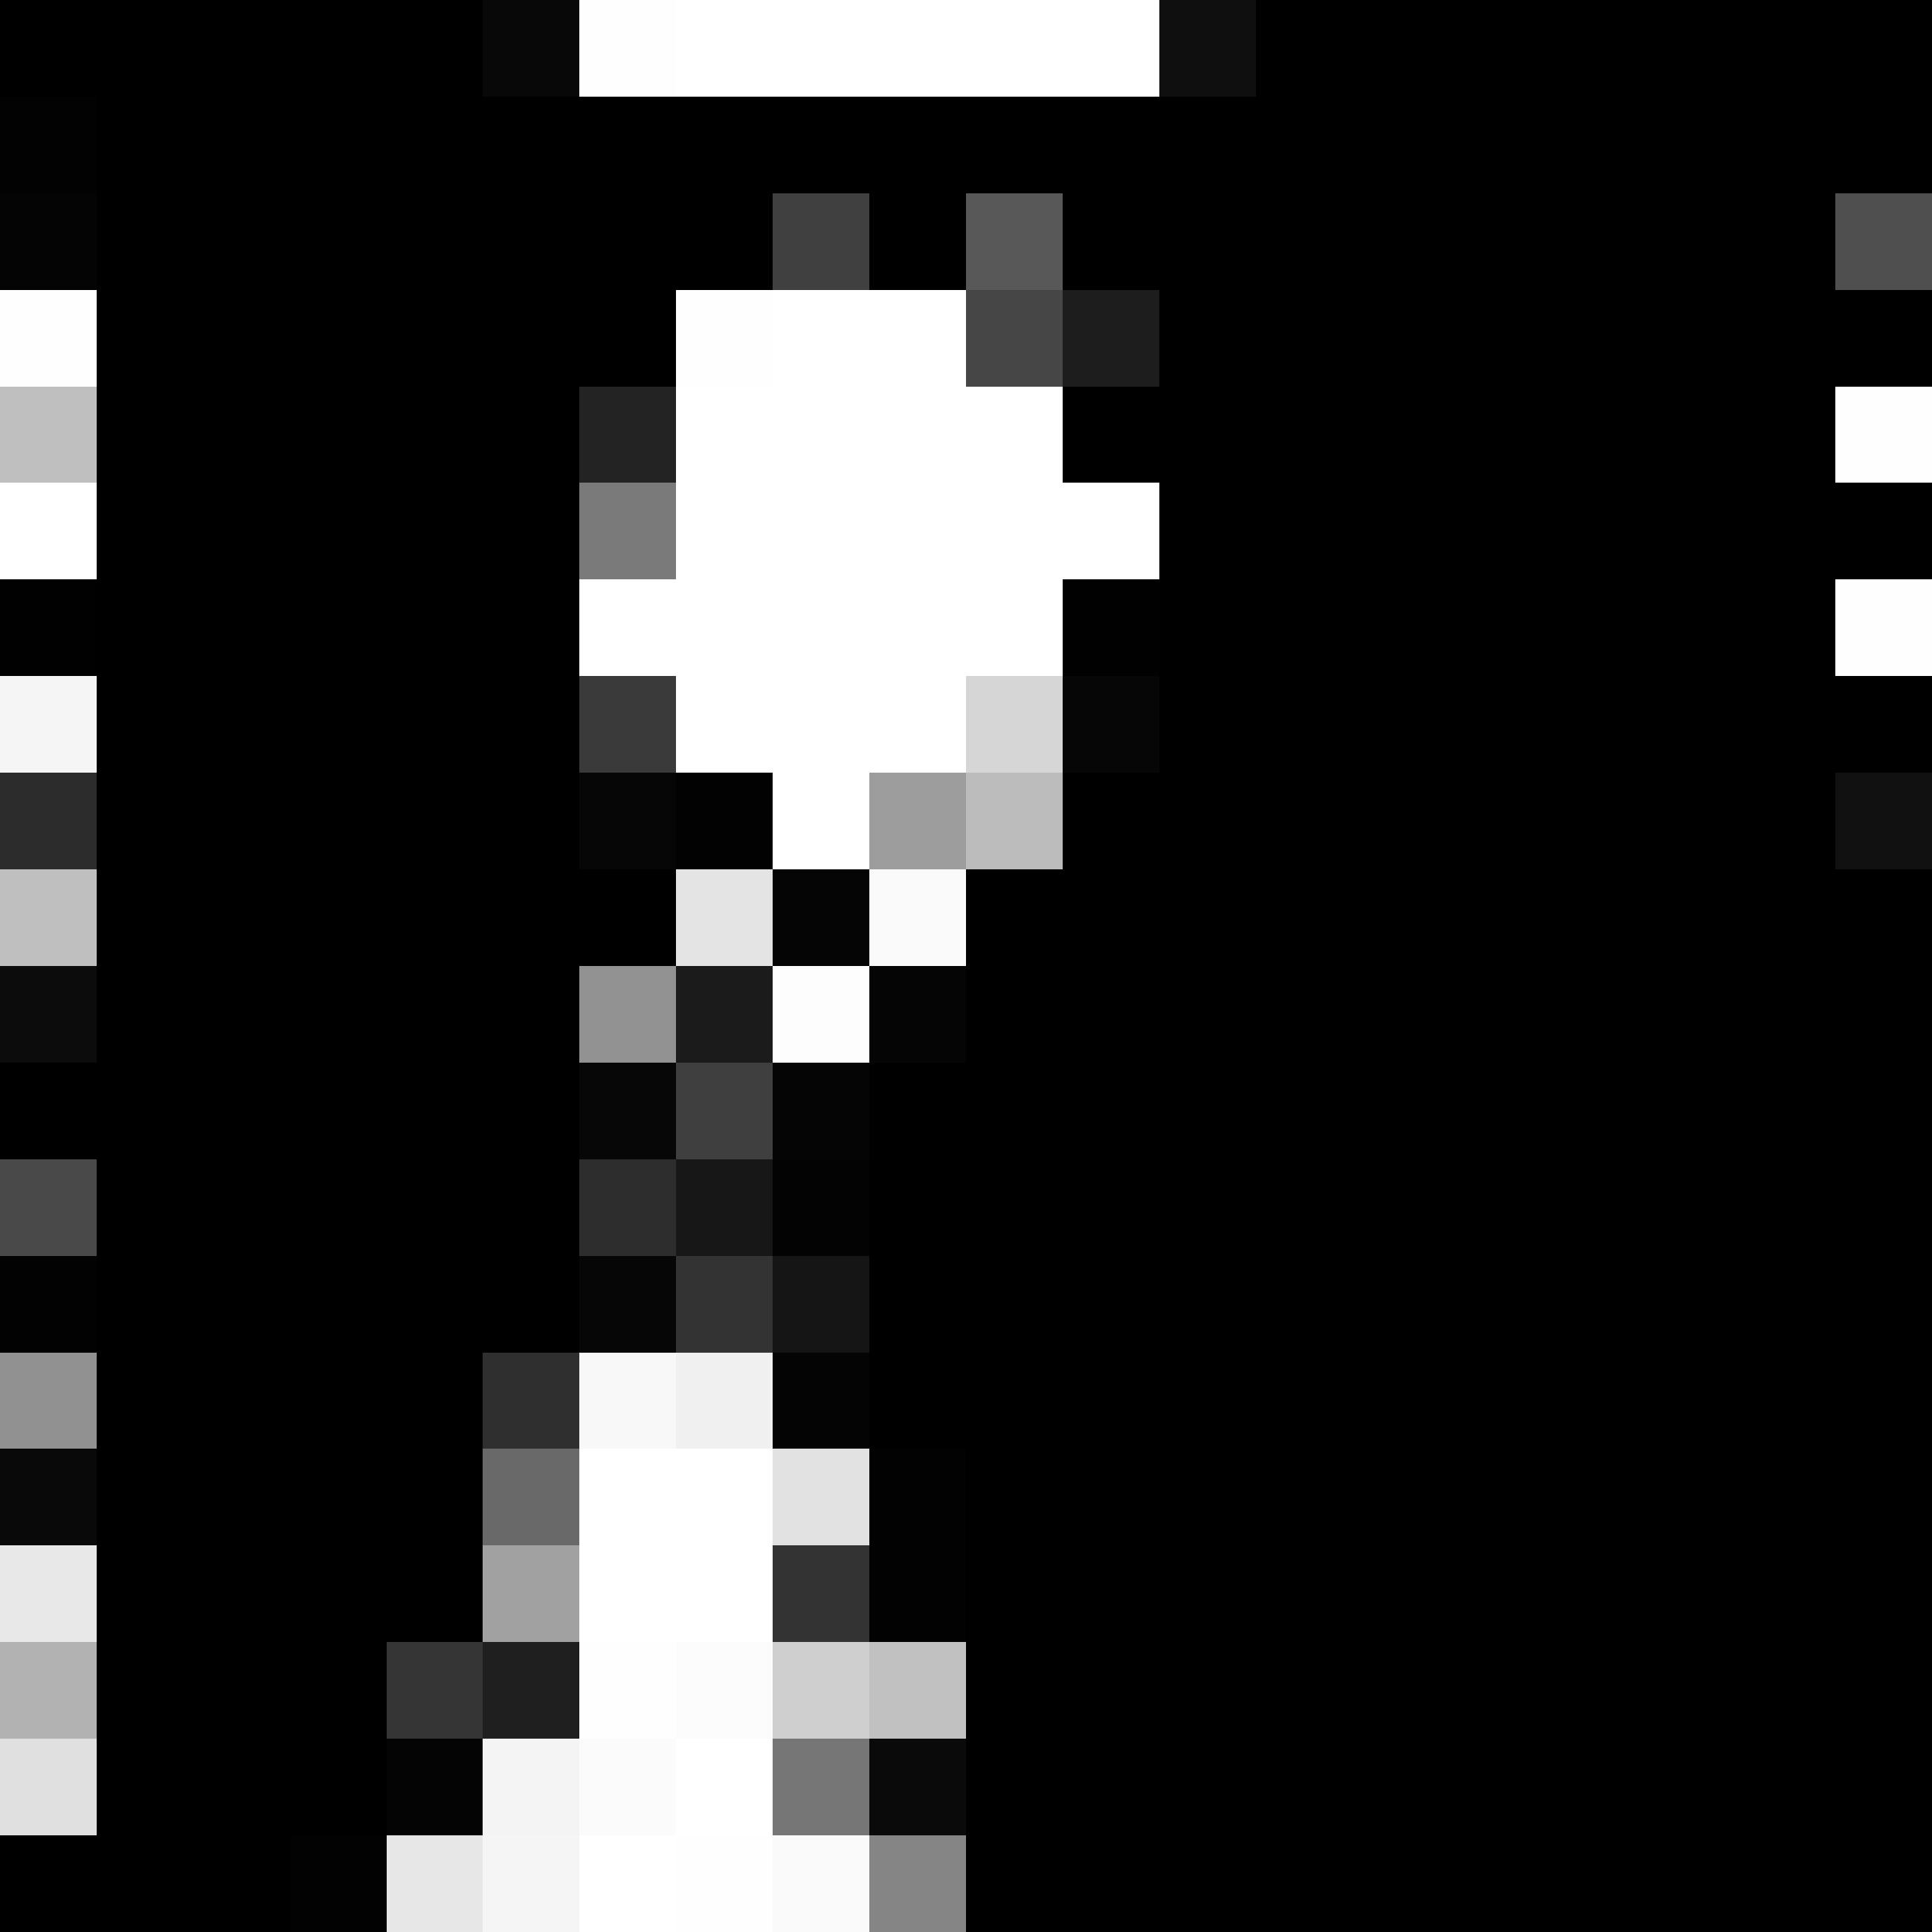
\includegraphics[width=\textwidth]{training_pc_3}
    \end{minipage}
    \vspace{0.3cm}
    \begin{minipage}{0.32\textwidth}
        \centering
        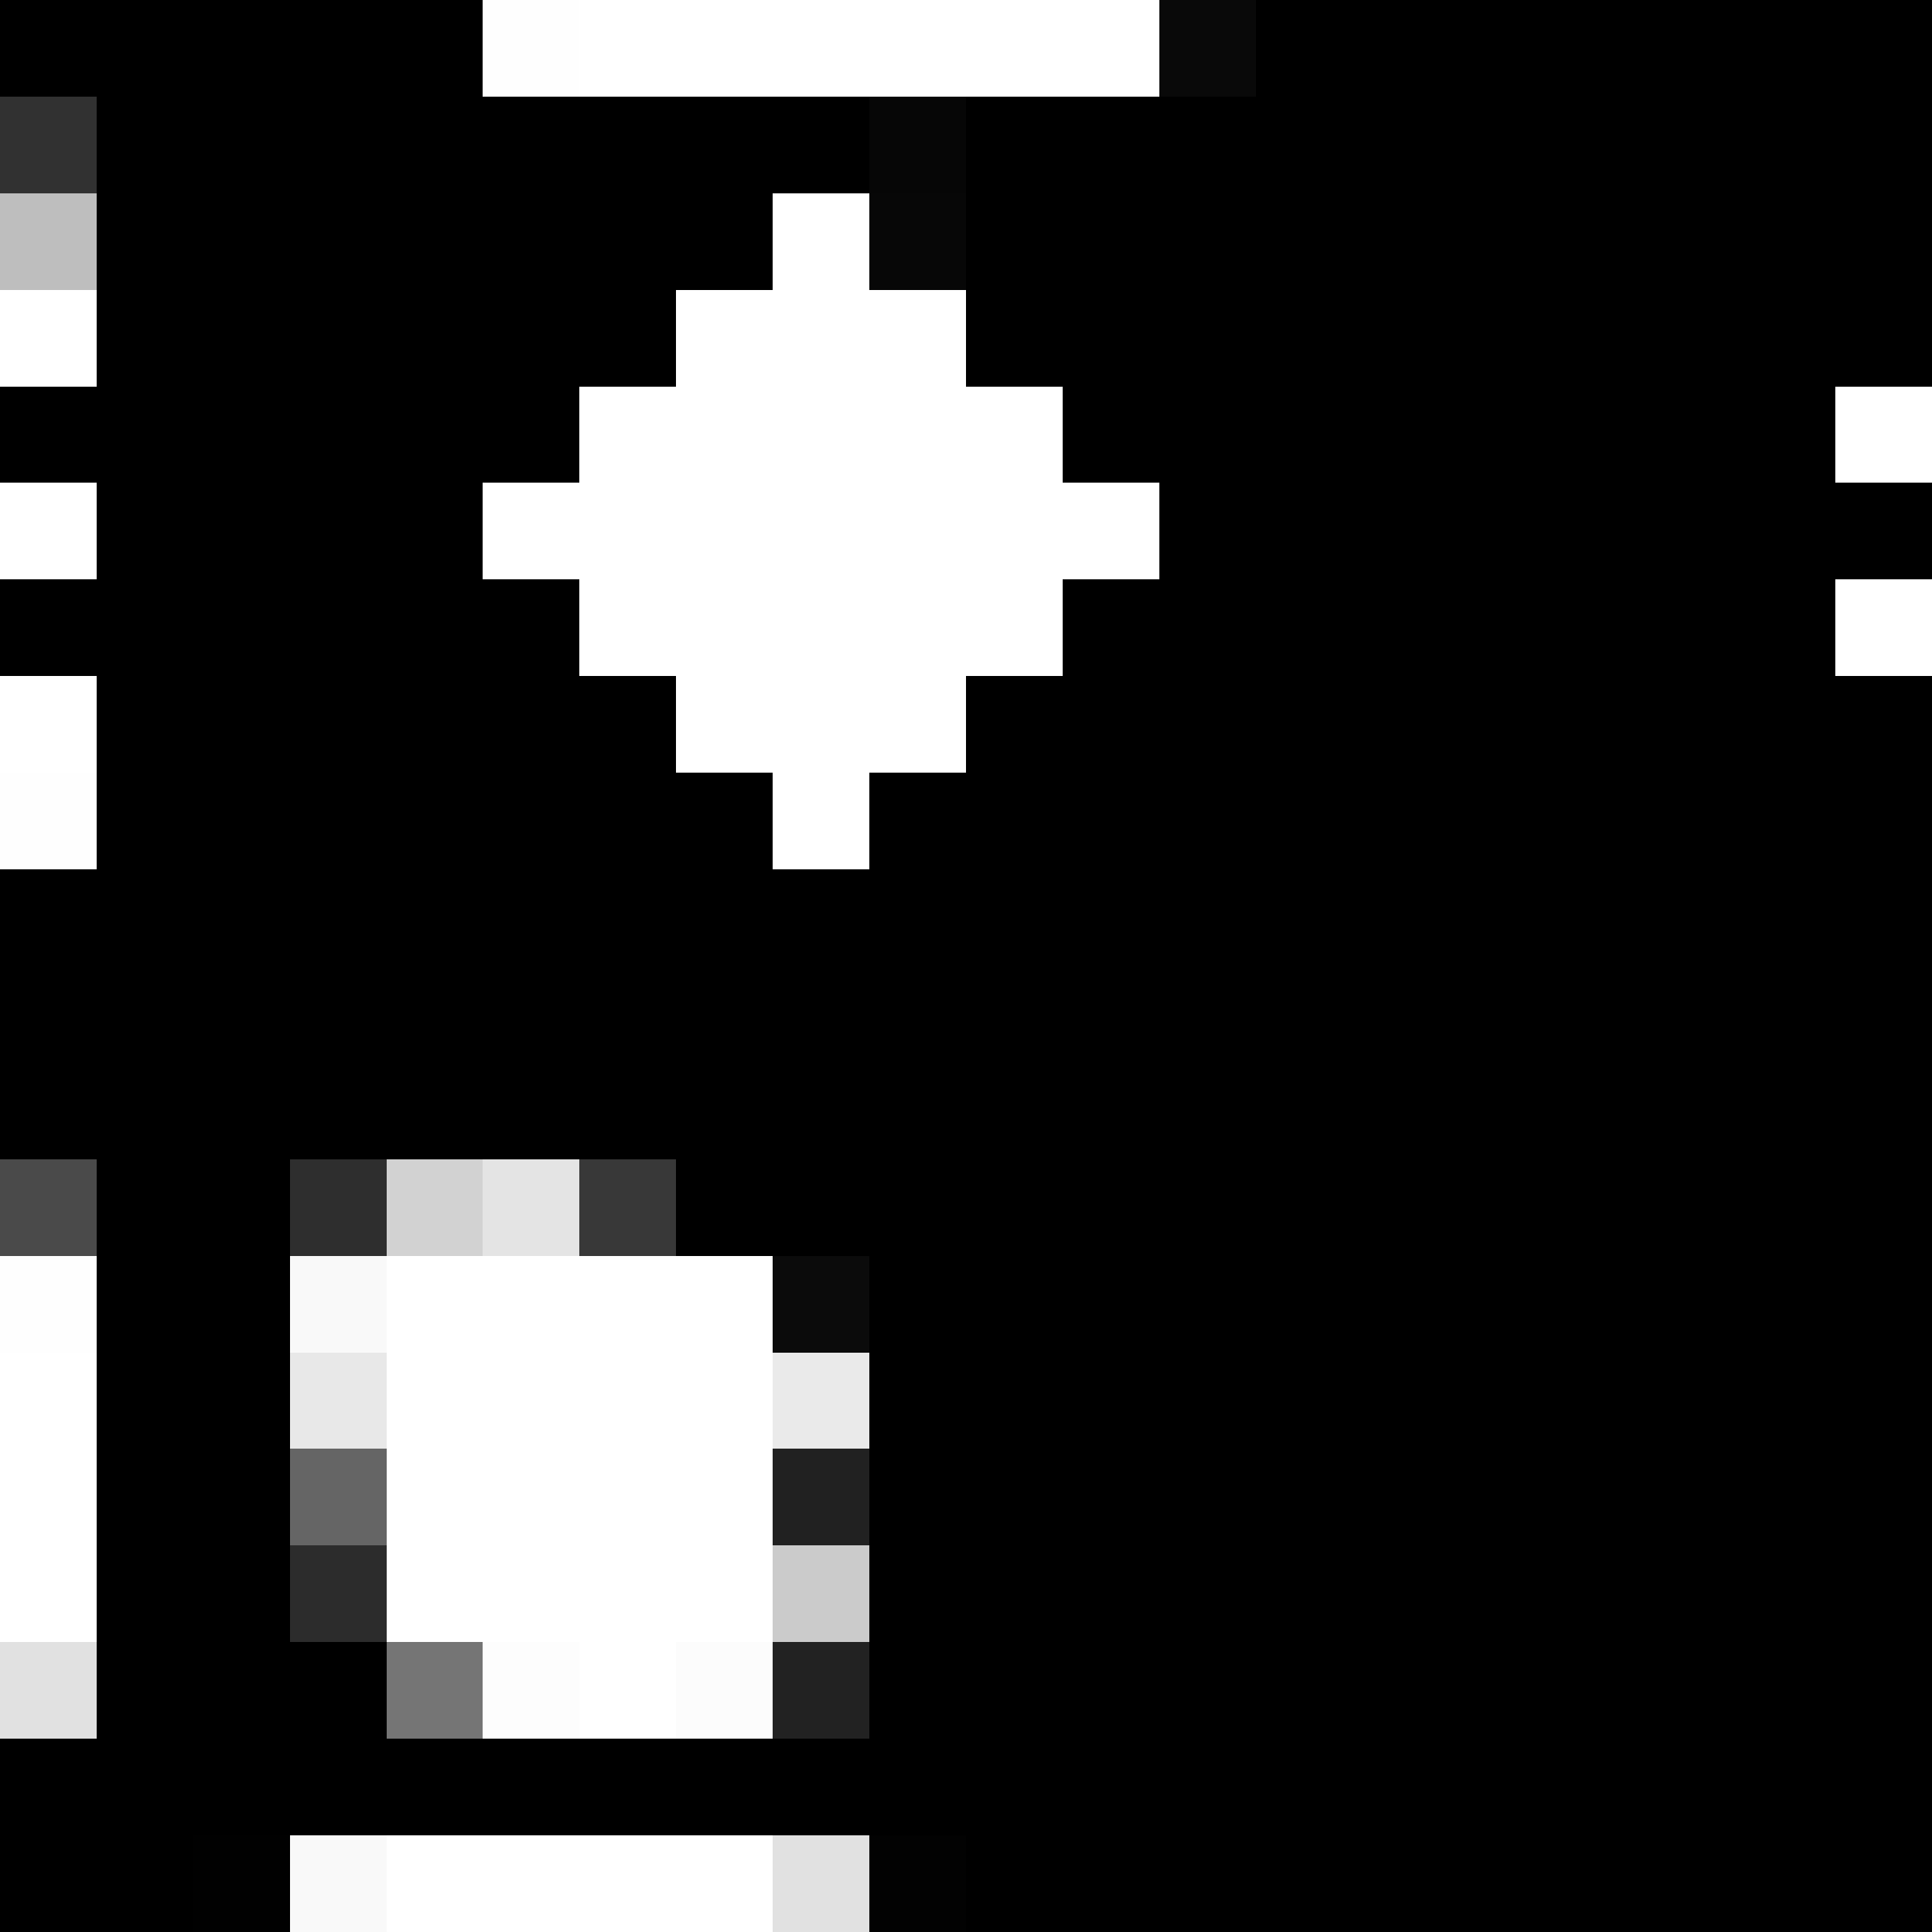
\includegraphics[width=\textwidth]{training_pc_4}
    \end{minipage}
    \begin{minipage}{0.32\textwidth}
        \centering
        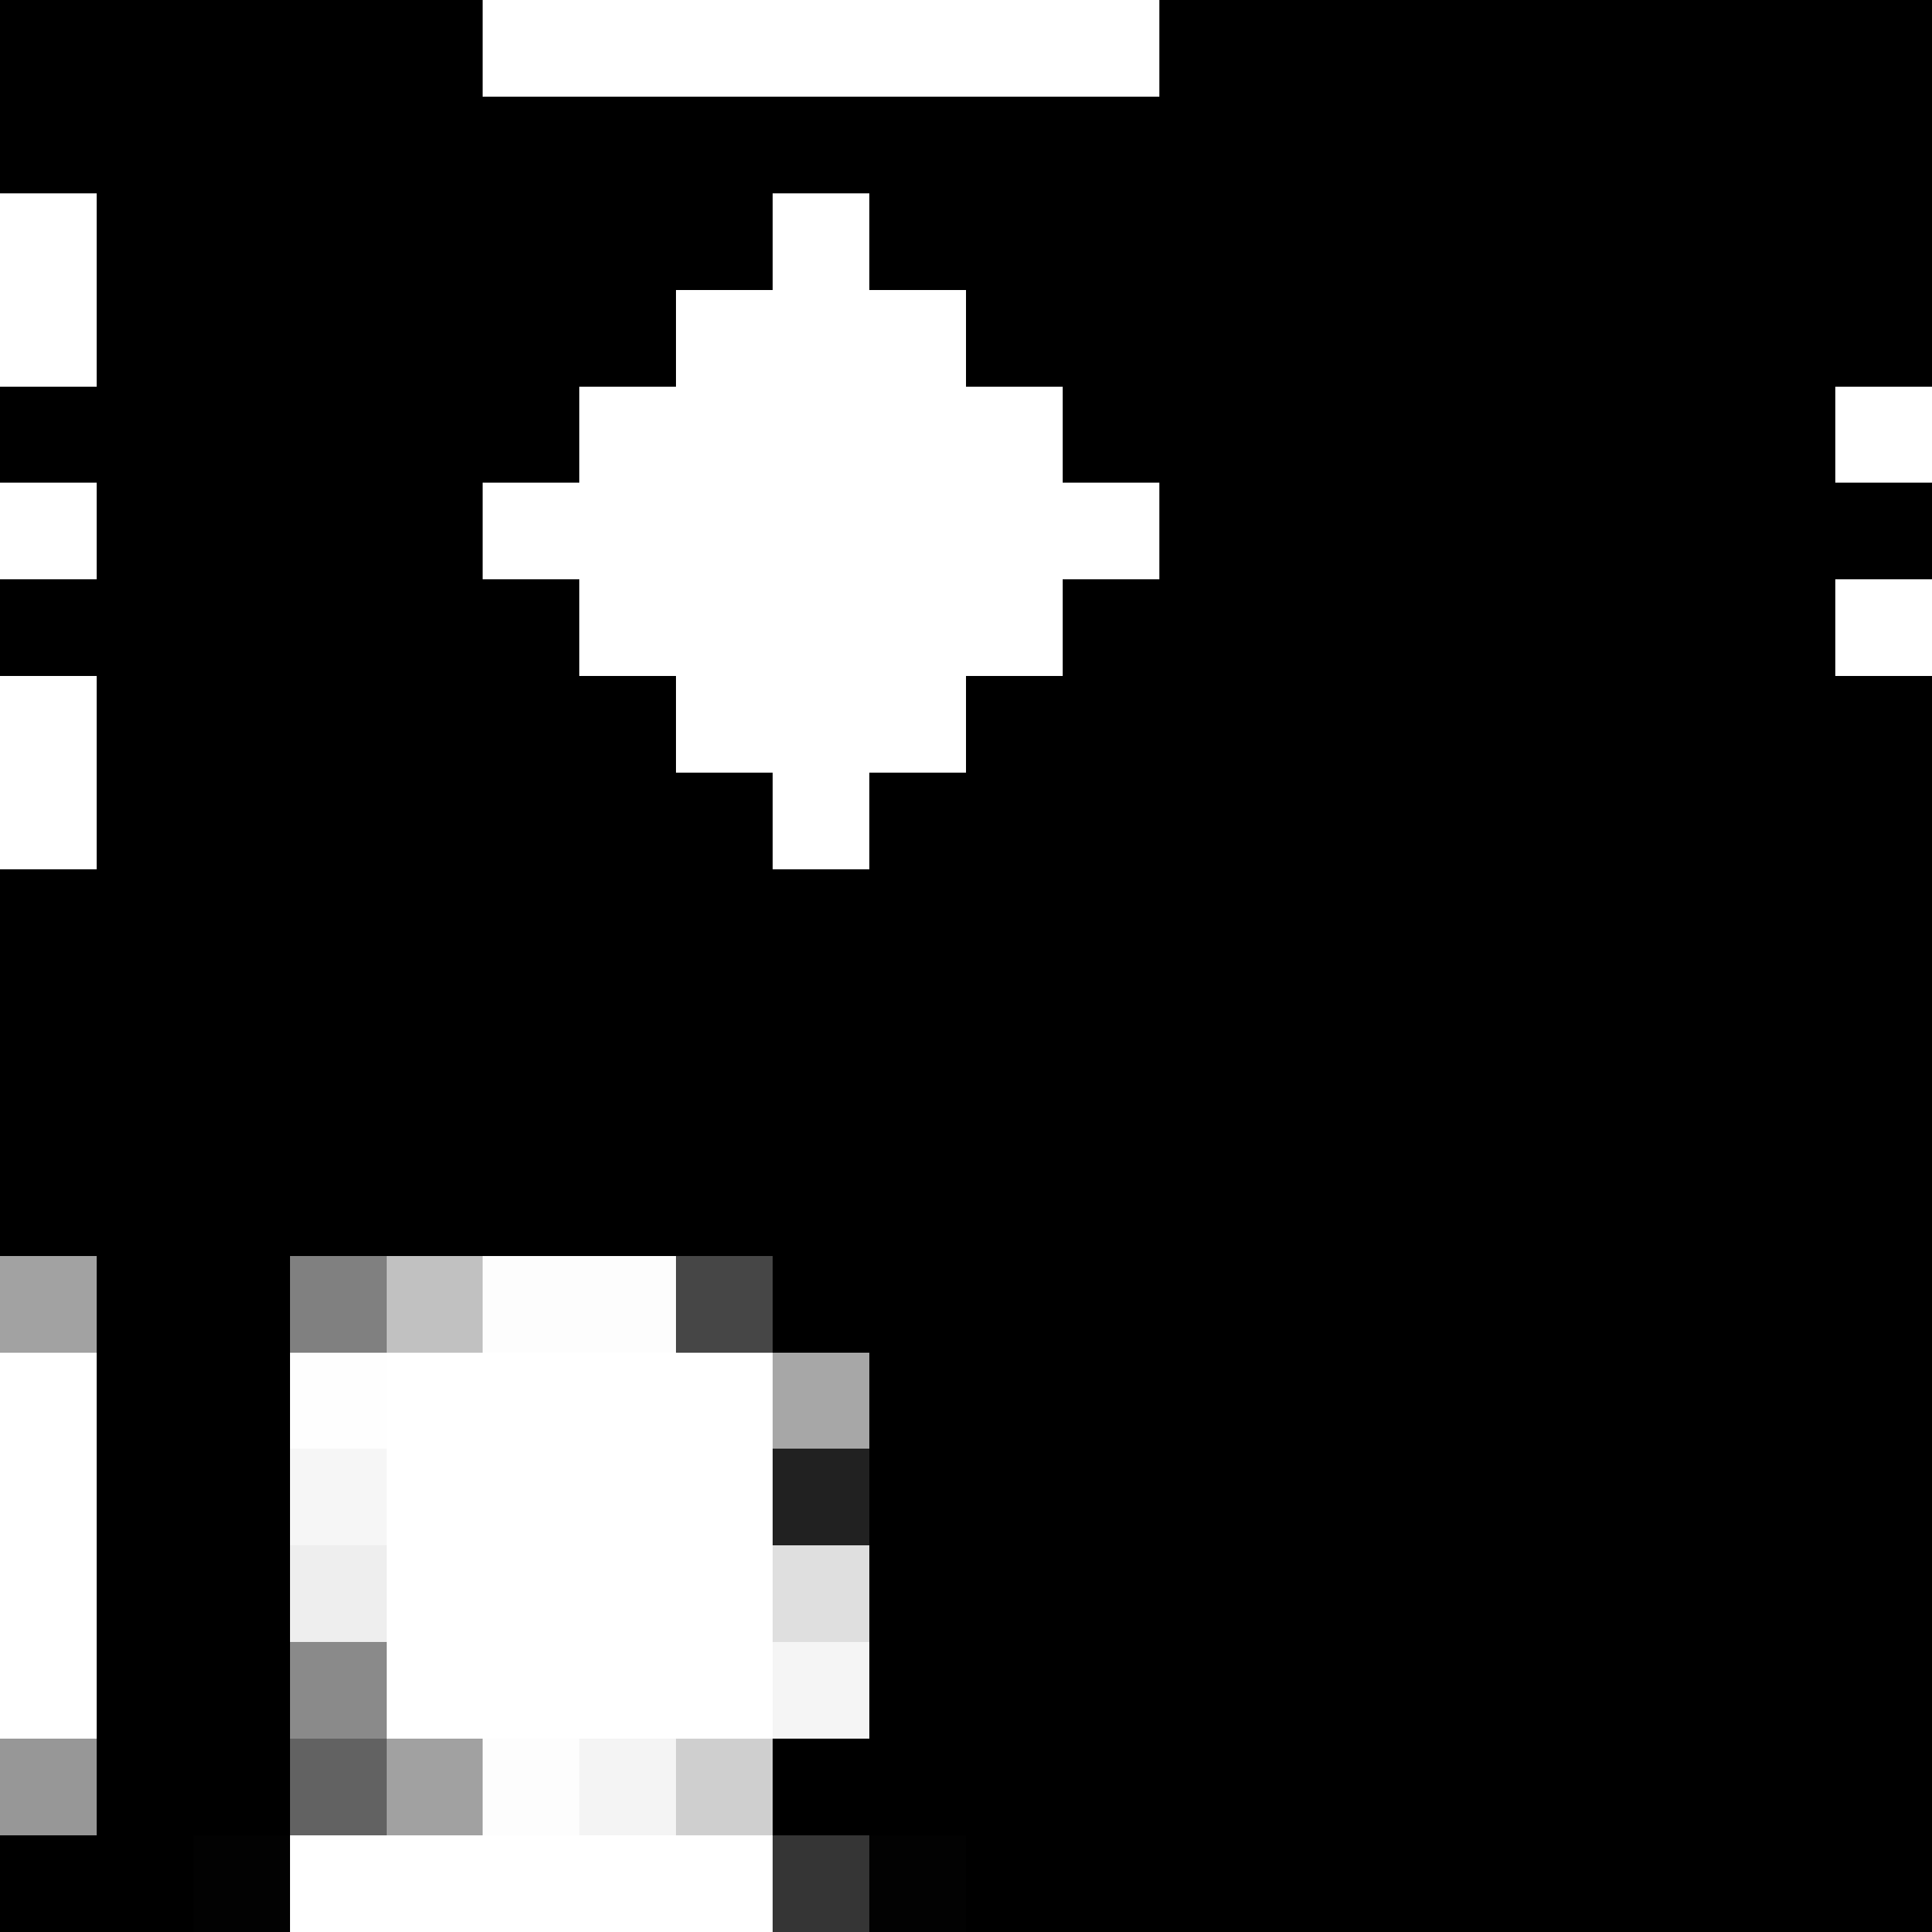
\includegraphics[width=\textwidth]{training_pc_5}
    \end{minipage}
    \begin{minipage}{0.32\textwidth}
        \centering
        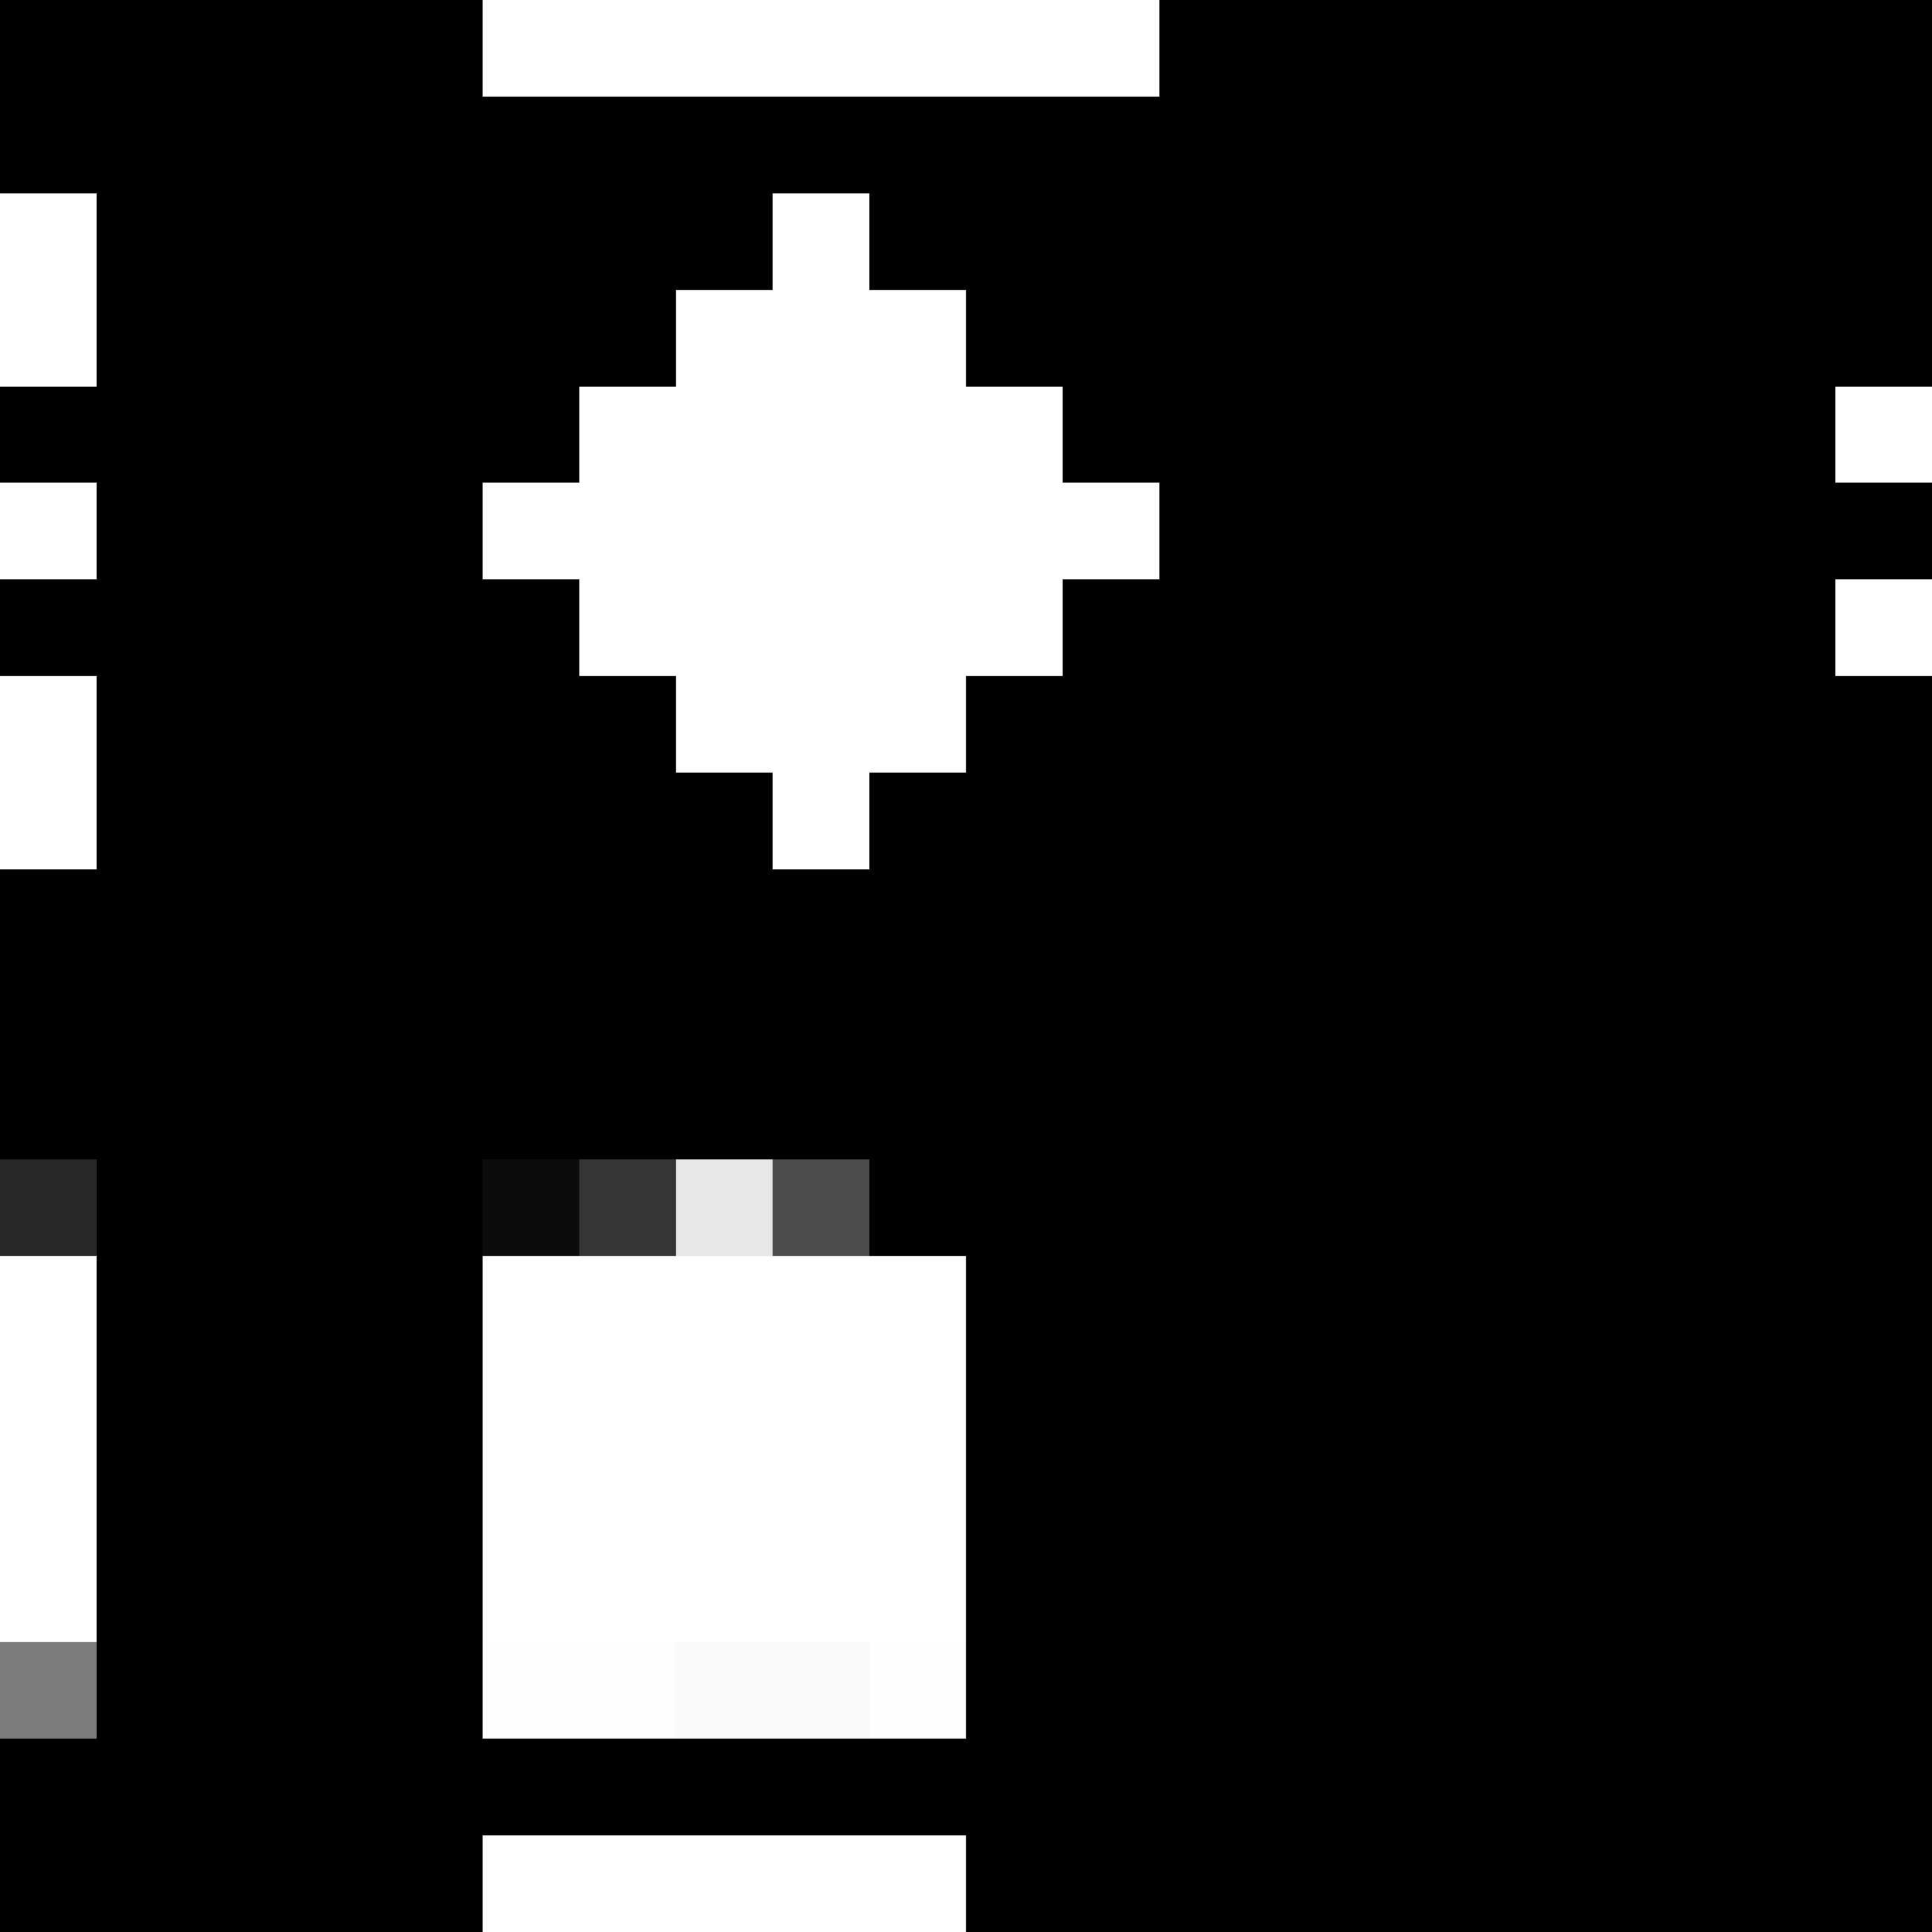
\includegraphics[width=\textwidth]{training_pc_6}
    \end{minipage}
    \caption{Samples drawn at different epochs from the generator trained on \textit{poly20\_pc} (zoom).}
\end{figure}
